\documentclass[a4paper,12pt]{article}
%\usepackage declarations should go here
\usepackage{graphicx}
\usepackage[T1]{fontenc}
\usepackage{parskip}
\usepackage{amsmath, amssymb, float, caption, algorithm, algorithmic, setspace}
\usepackage{natbib}
\usepackage{graphicx}
\usepackage{xcolor}
\usepackage{times}
\usepackage{zi4}
\usepackage[a4paper,left=2.5cm,right=2.5cm,top=2.5cm,bottom=3cm]{geometry}
\usepackage{hyperref}
\bibliographystyle{abbrvnat}
\setcitestyle{authoryear,open={(},close={)}}

%\usepackage{foundrysterlingbookosf}
  
\begin{document}
 
% Turn off page numbering until first section.
\pagenumbering{gobble}

% Title page - needs Stats_Logo.png
\begin{titlepage}
\begin{center}
\vspace{1cm}
\textsf{\Huge{University of Oxford \\}}
\vspace{1cm}
\begin{figure}[htb]
\centering

\includegraphics[scale=.8]{Stats_Logo.png}
\end{figure}
\vspace{2.0cm}
\Huge{Particle Markov Chain Monte Carlo for Integral Projection Models\\}
\vspace{2.0cm}
\large{ by \\[14pt] Calliste Fagard-Jenkin \\[8pt] St Cross College} \\
\vspace{2.2cm}
\large{A dissertation submitted in partial fulfilment of the degree of Master of Science in Statistical Science.
} \\
\vspace{.5cm}
\large{\emph{Department of Statistics, 24--29 St Giles, \\Oxford, OX1 3LB}} \\
\vspace{1.0cm}
\large{September 2019} \\
\end{center}
\end{titlepage}
\clearpage

This is my own work (except where otherwise indicated)
\vspace{2.5in}

\begin{center}
Candidate: Calliste Fagard-Jenkin\\
\vspace{1.0in}
Signed:.................................\\
\vspace{1.0in}
Date:...................................
\end{center}
\clearpage
\begin{abstract}


We explore the Integral Projection Model (IPM), a common tool in statistical ecology for use with census data. IPMs attempt to draw inference on the demography of trait-structured populations by fitting functions which describe the relationship between the size (mass, length, or other) of an individual and certain vital rates (such as its probability of survival, reproduction or growth to a given size). Traditionally, these functions are fitted piecemeal using the same data, by maximum likelihood estimation (MLE). This approach is unsatisfactory, as it is unable to elucidate parameter correlation structures, which is highly important for effective inference in the ecological sphere, where many complicated biological behaviours are interdependent. We propose a method making use of Particle Markov Chain Monte Carlo to produce Bayesian analyses of data sets whose structure is traditionally associated with IPMs. We favour this approach due to Gibbs samplers' weakness to mix well when parameters are highly correlated, because parameters are only updated in small sets at a time \citep{Finke}. Further to this, the use of particle filtering in Integrated Population Models is a relatively recent addition to the toolbox of ecological statisticians, with a recent pioneering paper by \citet{Finke}, which inspires the model specification we use. We apply our methodology to the analysis of both simulated and real Soay Sheep (\textit{Ovis aries}) data from Scotland. We conclude that the methodology shows promise in obtaining estimates of vital rate parameters with smaller, easier to collect data sets, allowing a robust exploration of the posterior correlation, and that the use of prior information is extremely important, as certain parameters become unidentifiable in the new parameterisation.

\end{abstract}
\clearpage
%\thispagestyle{empty}
\vspace*{2in}
\begin{center}
\textbf{Acknowledgements}
\end{center}

I would like to thank the project supervisors Prof. David Steinsaltz and Prof. Tim Coulson for their generous insight, support and patience, as well as Maria Christodoulou for her guidance and assistance with the guppy data, which was the initial candidate for the case study in section 5. I would also like to thank Prof. Michel Riguidel of the Ecole Nationale Superieure des Telecommunications and M. Willem Bonnaffe of the University of Oxford Department of Zoology, without whom I would not have been able to use this MSc as a springboard for further research.

\clearpage


\tableofcontents
\listofalgorithms
\listoffigures
\listoftables


\clearpage

\pagenumbering{arabic}

\section{Introduction}

Ecology is notorious for its complicated networks of interdependent species and the many layered ways in which they influence each other's demography. How then, in such a context, do we draw inference on the traits of a specific species of interest, or even track its demography over time? The use of the Matrix Projection Model, in which populations are divided into discrete classes according to certain traits, such as size, age or sex, has been a popular tool for analysing census data which have been collected over multiple breading seasons \textcolor{red}{[CITATION]}. Popularised by \citet{MatrixProjection}, these Matrix Projection models allow us to approximate the Leslie Matrix \citep{Leslie} of a population, which is an invaluable tool for predicting the growth rate of the population (determined by its leading eigenvalue) or the projected age or size distribution of the population over time (determined by the corresponding eigenvector). The Integral Projection Model (IPM) is conceptually identical to the Matrix Projection Model, and is simply a re-imagining of this which allows for continuous demographic traits.\\

The goal of the IPM is to specify a transition kernel which describes how the density of the population changes with respect to the distribution of the trait of interest from one time-step to the next. Whilst the trait of interest with respect to which the population is structured can in principle be anything (size, age, sex, etc.), we focus here on the size of individuals, as this is most relevant to the data set we hope to analyse, and is also the trait chosen by \citet{Ellner}; an introductory work on the Integral Projection Model from which we replicate a case study later in this dissertation. \\

The IPM kernel must assume a fixed order of events for the life cycle of individuals in between censuses. In our case, we assume that the first event is survival of the individual (or lack thereof), followed by growth of the individual, and then reproduction. There are plenty of other possible life cycles, but we note our preference for this specification for similar reasons. \\

Using the above described life cycle order, and therefore assuming that all censuses take place soon after reproduction, we obtain the following transition kernel for the IPM \citep{Ellner}:

\begin{equation}
    K(z^{'}, z) = s(z)G(z^{'}, z) + s(z)p_b(z)b(z)C_1(z^{'},z)/2
\end{equation}

Where $z^{'}$ refers to the size of an individual at the current census, and $z$ to the size of an individual at the previous census. The kernel is split up into two terms. The first gives us the density of individuals present in the population because they have survived from the previous census, and the second term gives us the density of individuals entering the population by being birthed by parents that survived from the previous census, and reproduced. The left hand term of the kernel describes the probability of an individual surviving from the previous census to the current one ($s(z)$) and the probability the individual grows from its previous size $z$ to its current size $z^{'}$ ($G(z^{'}, z)$). The right hand term of the kernel then consists of the probability that the individual of size $z$ survives, reproduces ($p_b(z)$), produces a number of children distributed $b(z)$ and that the probability the child is of size $z^{'}$ ($C_1(z^{'},z)$). We include the factor of $\frac{1}{2}$ since this dissertation will focus on models that only track the females in the population, for simplicity, but formulating an IPM that tracks both sexes involves only a minor modification to the parameterisation (for example, the probability of reproduction in the kernel would now include a term for the probability that the individual is female). This kernel defines the IPM which describes the change in the size distribution of the population from one census to the next \citep{Ellner}:

% KERNEL EQUATION %
\begin{equation}
    n_{t+1}(z') = \int_L^U K(z^{'}, z)n_t(z)dz
\end{equation}

Where $n_{t}(x)$ gives the density of individuals in the population that have size $x$ at time $t$, and where $L$ and $U$ are the lower and upper limits of the size of individuals, respectively. \\


IPMs are still widely solved by estimating the parameters of the vital rate functions in a piecemeal fashion e.g. \citet{Snakes, ThreatenedHerb, Struck, NichePlants, Quintana}. We suggest that this is potentially problematic when parameter values are correlated (which can easily be the case when population demography is changing over time \textcolor{red}{[CITATION]}), as Maximum Likelihood Estimation offers no information on the correlation structure of the parameters, when these functions are solved piecemeal. We suggest that on top of estimating these parameter values simultaneously, a Bayesian approach introduces multiple invaluable benefits, including the ability to more readily combine multiple data sets into the analysis, making use of prior information when sample sizes are small, and most importantly, incorporating covariance between vital rates \citep{BayesIPM}.\\

We suggest that exploring parameter correlation is important, due to this phenomenon being a natural consequence of most biological behaviour. As an example, we consider the case where the quantity of resources (such as food) vary from year to year. A year with abundant resources would intuitively lead to a potential increase in both survival rate and growth rate, introducing temporal correlation between these vital rates. Using a naive IPM formulation would not allow us to account for this, even when fitting vital rate functions simultaneously, without complicating the model specification. Whilst it may be possible to incorporate this correlation into the uncertainty of estimates of interest (via a bootstrap which resamples parameter values from their asymptotic normal distribution, for example) we argue that a Bayesian framework leads to this result more directly, and allows us to draw more robust inference on these parameters, and any statistics of interest derived thereof.

\newpage
\section{Piecemeal Solving}
% THE INDIVIDUAL BASED MODEL %
\subsection{The Individual Based Model}
 Before we give an example of piecemeal solving, we briefly introduce an Individual Based Model (IBM) to simulate observations, which can then be used to fit IPMs. This allows us to draw data from a population with known behaviour, so that we may more effectively compare the efficacy of the different solving methods and algorithms at our disposal. The IBM iterates through each individual in the population at every time step, determining firstly if it survives, and then (conditionally on survival) it determines its new size, whether or not it reproduces, and the size of its offspring. An example of the type of data this process generates is given by Table \ref{tab:DataExampleIBM}:\\


% latex table generated in R 3.5.1 by xtable 1.8-4 package
% Wed Aug 07 14:45:21 2019
\begin{table}[ht]
\begin{center}
\resizebox{\linewidth}{!}{%
\begin{tabular}{cccccccccc}
  \hline
 individual & size & survived & census.number & parent.size & reproduced & prev.size & off.survived & off.born \\ 
  \hline
 1 & 2.77 & 1 & 1 & 3 & NA & NA & NA & NA \\ 
   2 & 2.72 & 1 & 1 & 3 & NA & NA & NA & NA \\ 
   3 & 2.37 & 1 & 1 & 3 & NA & NA & NA & NA \\ 
   4 & 2.37 & 1 & 1 & 3 & NA & NA & NA & NA \\ 
  5 & 2.39 & 1 & 1 & 3 & NA & NA & NA & NA \\ 
  \hline
   1 & 3.06 & 1 & 2 & NA & 1 & 2.77 & 1 & 1 \\ 
   2 & 3.02 & 1 & 2 & NA & 1 & 2.72 & 1 & 1 \\ 
   3 & 2.73 & 1 & 2 & NA & 1 & 2.37 & 1 & 1 \\ 
   4 & 2.79 & 1 & 2 & NA & 0 & 2.37 & NA & NA \\ 
   5 & 2.83 & 1 & 2 & NA & 1 & 2.39 & 1 & 1 \\ 
   6 & 2.17 & 1 & 2 & 2.72 & NA & NA & NA & NA \\ 
   7 & 2.33 & 1 & 2 & 2.37 & NA & NA & NA & NA \\ 
  \hline
   1 & 3.09 & 1 & 3 & NA & 1 & 3.06 & 1 & 1 \\ 
   2 & 3.12 & 1 & 3 & NA & 1 & 3.02 & 1 & 1 \\ 
   3 & 2.89 & 1 & 3 & NA & 0 & 2.73 & NA & NA \\ 
   4 & 2.98 & 1 & 3 & NA & 1 & 2.79 & 1 & 1 \\ 
   5 & 3.05 & 1 & 3 & NA & 0 & 2.83 & NA & NA \\ 
   6 & NA & 0 & 3 & NA & NA & 2.17 & NA & NA \\ 
   7 & 2.78 & 1 & 3 & NA & 1 & 2.33 & 1 & 1 \\ 
   8 & 2.19 & 1 & 3 & 2.33 & NA & NA & NA & NA \\ 
   \hline
\end{tabular}
}
\end{center}
\caption{\label{tab:DataExampleIBM}Example data simulated from the IBM, consisting of a survey of 3 censuses, with a starting population of 5 individuals.}
\end{table}

\vspace{0.5cm} % padding for table %

Table \ref{tab:DataExampleIBM} is an excellent example of the format of real-world data that we obtain to fit IPMs. Each individual in our population is given a unique ID, which we keep track of using the first column. The `survived' column is an indicator for the presence of the individual in the current survey, which is taken to mean survival. In some cases individuals are not perfectly detected, and so we could choose to incorporate this into our model so that the probability of observing an individual becomes the product of the probability of survival and the probability of detection. We can see that individuals who have not survived are recorded as having size NA in the census before they died, since the size was unobserved due to the individual's absence from the census. The `parent.size' column only includes the size of the parent of the individual for the census before which the individual was born, otherwise this column contains an NA. Similarly, if an individual is deceased or newly born, its reproduced column has value NA (this introduces the assumption that the intervals between censuses are small enough that a newly born individual does not reach sexual maturation before it is censused for the first time). The `off.born' column (the number of offspring born engendered by the parent on the given row of the data) is often impossible to obtain when conducting real world data, but represents the total number of offspring in the litter of a given parent.

% VITAL RATE SPECIFICATION %
\subsection{Specification of Vital Rate Functions}
The survival of an individual from one census to the next is modelled by a Bernoulli distribution:

\begin{equation}
    \text{logit}(p_{i,t}) = p_0 + p_1 \cdot \text{size}_{i, t-1}
\end{equation}\\

Where $p_{i,t}$ gives the probability that individual $i$ has of surviving from the census at time $t-1$ to the census at time $t$, given $\text{size}_{i, t-1}$, its size at the census $t-1$. All individuals survive independently of each other, such that the likelihood of the survival of all individuals across all censuses is:

% SURVIVAL LIKELIHOOD %
\begin{equation}
    \mathcal{L}_{survival}(\boldsymbol{\mathcal{A}}|\boldsymbol{\mathcal{S}}, \boldsymbol{p}) = \prod_{i=1}^n\prod_{t=2}^T \left\{p_{i,t}^{\mathcal{I}(\text{alive}_{i, t})} \cdot (1-p_{i,t})^{\left(1-\mathcal{I}(\text{alive}_{i, t})\right)}\right\}^{\mathcal{I}(\text{alive}_{i, t-1})}
\end{equation}

Where there are $n$ unique individuals observed throughout the whole study and $T$ censuses conducted in total. $\mathcal{I}(\text{statement})$ is the standard indicator function, equal to 1 when the $\text{statement}$ is true, and 0 otherwise. $\text{alive}_{i, t}$ is a statement which is true when individual $i$ is alive at census number $t$, and is false otherwise. $\boldsymbol{\mathcal{A}}$ is the matrix which contains all of the $\text{alive}_{i, t}$ values, and is therefore mostly sparse. Similarly, $\boldsymbol{\mathcal{S}}$ is the matrix containing all of the $\text{size}_{i,t}$ values. $\boldsymbol{p}$ is the vector containing $p_0$ and $p_1$.

Given survival, the growth of an individual is given by a normal distribution, centred at a linear projection of the size at the previous census, and truncated on both tails to remain within the specified lower and upper bounds of the possible size of individuals:

% GROWTH LIKELIHOOD %
\begin{equation}
            \mathcal{L}_{\text{growth}}(\textbf{S} |\boldsymbol{\mathcal{A}}, \boldsymbol{\mu}, \sigma^2) = \prod_{i=1}^n \prod_{t=2}^T \left\{\frac{\phi(\text{size}_{i, t}, \mu_{i,t}, \sigma^2)}{\Phi(U,\mu_{i, t},\sigma^2)-\Phi(L,\mu_{i, t},\sigma^2)}\right\}^{\mathcal{I}(\text{alive}_{i, t}) \cdot \mathcal{I}(\text{alive}_{i, t-1})} \\
\end{equation}

\begin{equation}
    \mu_{i, t} = \mu_0 + \text{size}_{i, t-1} \cdot \mu_1
\end{equation}

Where $\phi$ is the probability density function of the normal distribution evaluated at the first argument, given its mean and variance as the following two arguments, and where $\Phi$ is its cumulative distribution function. This parameterisation assumes that the lower and upper bounds of the size variable (L and U, respectively) are chosen sensibly, such that all observations are contained within the interval [L,U].

We consider each individual to have an independent probability of reproducing between each census, which depends only on the size of the individual at the previous census. This gives it the same formulation as $\mathcal{L}_{\text{survival}}$ with different indicator functions and parameter values:

% REPRODUCTION LIKELIHOOD %
\begin{equation}
    \mathcal{L}_{\text{reproduction}}(\boldsymbol{\mathcal{R}}|\boldsymbol{\mathcal{S}}, \boldsymbol{\mathcal{A}}, \boldsymbol{p}) = \prod_{i=1}^n\prod_{t=2}^T \left\{p_{i,t}^{\mathcal{I}(\text{reproduced}_{i, t})} \cdot (1-p_{i,t})^{\left(1-\mathcal{I}(\text{reproduced}_{i, t})\right)}\right\}^{\mathcal{I}(\text{alive}_{i, t-1})}
\end{equation}

Given that the individual reproduces, we consider the number of offspring it engenders to be Poisson distributed, truncated so that only non-zero quantities of offspring are allowed. This leads to the following likelihood function:

% OFFSPRING COUNT LIKELIHOOD %
\begin{equation}
    \mathcal{L}_{\text{offspringCounts}}(\boldsymbol{\mathcal{C}}| \boldsymbol{\mathcal{A}}, \lambda) =  \prod_{i=1}^n\prod_{t=2}^T \left\{\frac{\lambda^{\mathcal{C}_{i, t}}e^{-\lambda}}{\mathcal{C}_{i, t}!}\left[\int_1^{\infty}\frac{\lambda^{\mathcal{C}_{i, t}}e^{-\lambda}}{\mathcal{C}_{i, t}!}d\mathcal{C}_{i, t}\right]^{-1}\right\}^{\mathcal{I}(\mathcal{C}_{i, t}>0)\cdot\mathcal{I}(\text{alive}_{i, t})\cdot\mathcal{I}(\text{reproduced}_{i, t})}
\end{equation}

Where $\mathcal{C}_{i,t}$ is the number of offspring engendered by individual $i$ between census $t-1$ and census $t$. $\lambda$ is the average number of children per individual (when they reproduce, and constant for the whole population). If litter size rates were not constant throughout the population, we could equally turn $\lambda$ into some $\lambda_{i, t} = \lambda_0 + \text{size}_{i, t}$ (for example) if so desired.

The size of offspring at first census is taken to have the same form as $\mathcal{L}_{\text{growth}}$, with different parameter values. That is, we assume that the size of a newborn individual at first census is normally distributed around the weight of its parent.

Occasionally we also introduce infant mortality, as per Table \ref{tab:DataExampleIBM}, such that an offspring surviving to the first census after its birth follows a Bernoulli distribution.

\subsection{Fitting the Vital Rate Functions}
% FITTING VITAL RATE FUNCTIONS %

We replicate a case study in \citet{Ellner} to illustrate the process of estimating the parameters of the vital rate functions. This case study consists of the analysis of simulated data, which reflects the behaviour of a population of feral Soay Sheep (\textit{Ovis  aries}) based on the island of Hirta off of the northwest Coast of Scotland \citep{Ellner}. We include the truncation of the specified vital rate functions during simulation of the data set, but obtain maximum likelihood estimates using only Generalised Linear Models (GLM) and Linear Models (LM), to better reflect common practice in recent literature \citep{Snakes, ThreatenedHerb, Struck, NichePlants, Quintana}).\\


We simulate the data tracking only the females in the population, with a starting population size of 500. We allow the simulation to progress from census to census, until the population size reaches 5000 females, which leads to a survey of 109 censuses. To better reflect the uncertainty of real-world data collection, and to remain consistent with the example given in \citet{Ellner}, a random sample of 3000 individuals from only the final census is used for the analysis. The simulation assumes that reproduction always leads to the birth of a single individual, and so we do not simulate or estimate random litter sizes, as per equation (8). The size of the individuals is reported as mass of the individual on the log scale. \\

\begin{figure}[H]
\begin{center}
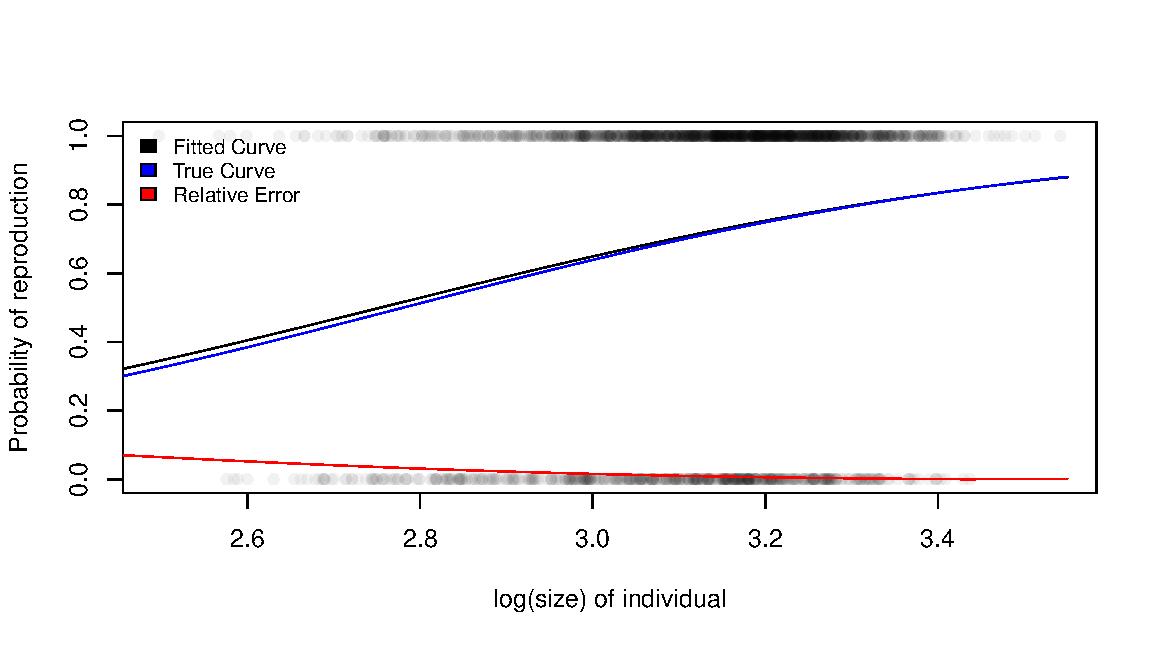
\includegraphics[scale=0.85]{UngulateReprIPM.pdf}
\caption{\label{ungRepIPM}Estimated and true reproductive probability functions for the simulated \textit{Ovis aries} data, with percentage error overlain.}
\end{center}
\end{figure}

\begin{figure}[H]
\centering
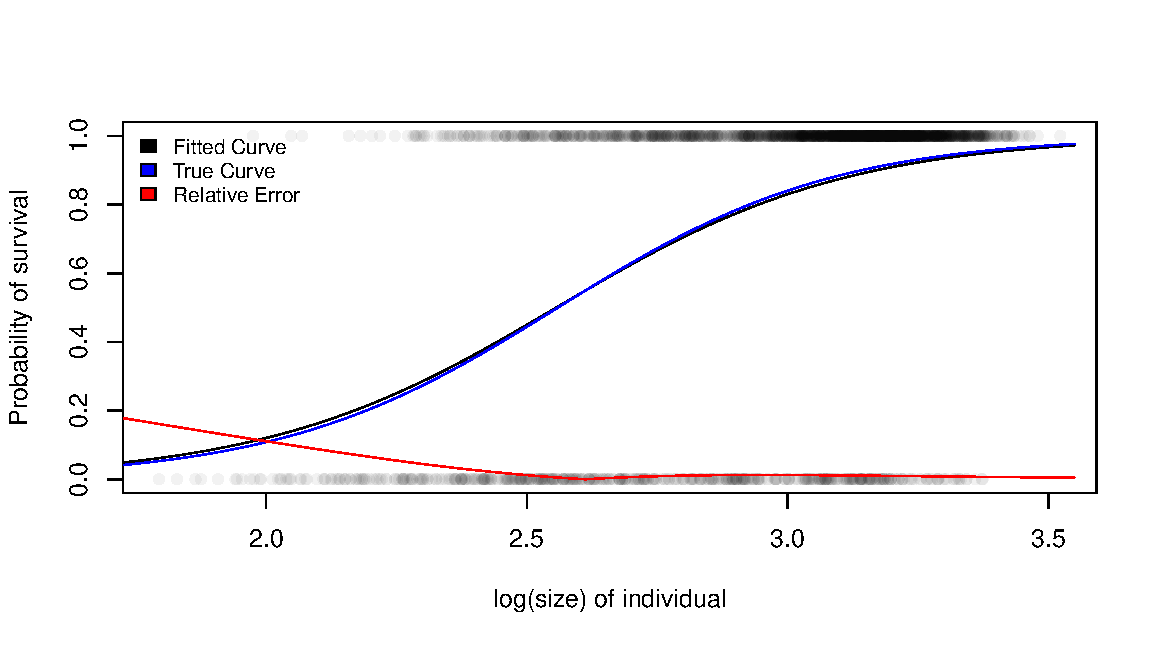
\includegraphics[scale=0.85]{UngulateSurvIPM.pdf}
\caption{\label{ungSurIPM}Estimated and true survival probability functions for the simulated \textit{Ovis aries} data, with percentage error overlain.}
\end{figure}

The parameters of the survival function are estimated using a binomial GLM, as are those of the reproduction function. The parameters of the growth and offspring sizes at first census functions are solved with a regular Linear Model, and the probability of survival of offspring to the first census is also solved using a binomial GLM. Figures \ref{ungRepIPM} and \ref{ungSurIPM} illustrate the fitted reproduction function and survival function, as a means to visualise the accuracy which we obtain from sampling 3000 individuals from the final census.\\

The estimated values of all parameters are given by tables \ref{OvisPars} and \ref{OvisTruncPars}:\\

% latex table generated in R 3.5.2 by xtable 1.8-4 package
% Sat Aug 17 09:19:28 2019
\begin{table}[ht]
\centering
\begin{tabular}{rrrrrr}
  \hline
 & \textbf{survival.i} & \textbf{survival.g} & \textbf{repro.i} & \textbf{repro.g} & \textbf{offsurv.p} \\ 
  \hline
 True Value & -9.6500 & 3.7700 & -7.2300 & 2.6000 & 0.8730 \\ 
  MLE & -9.1442 & 3.5764 & -6.8851 & 2.4996 & 0.8561 \\ 
   \hline
\end{tabular}
\caption{\label{OvisPars}Maximum Likelihood Estimates for the \textit{Ovis aries} simulated data, using 3000 sampled individuals from the final census}
\end{table}

\vspace{0.6cm}

% latex table generated in R 3.5.2 by xtable 1.8-4 package
% Sat Aug 17 09:25:51 2019
\begin{table}[ht]
\centering
\begin{tabular}{rrrrrrr}
  \hline
 & \textbf{growth.i} & \textbf{growth.g} & \textbf{growth.sd} & \textbf{offsize.i} & \textbf{offsize.g} & \textbf{offsize.sd} \\ 
  \hline
True Value & 1.4100 & 1.5600 & 0.0800 & 0.3600 & 0.7100 & 0.3600 \\ 
  MLE : No Truncation & 1.3999 & 0.5647 & 0.0803 & 0.3561 & 0.7098 & 0.1604 \\ 
  MLE : Truncation & 1.3993 & 0.5649 & 0.0803 & 0.3552 & 0.7101 & 0.1602 \\ 
   \hline
\end{tabular}
\caption{\label{OvisTruncPars}Maximum Likelihood Estimates for the parameters of the normally distributed vital rates of the \textit{Ovis aries} simulated data, using 3000 sampled individuals from the final census.}
\end{table}

As Table \ref{OvisTruncPars} illustrates, there is only a marginal difference between using a truncated or typical normal distribution when estimating the MLEs of the growth and offspring size functions. However, it should be noted that this is because the parameter values we simulate the data from place little probability mass on the tails of the distribution. In situations where realistically modelling real world behaviour would require truncating significant portions of the probability mass, it would be advised to compare parameter estimates with and without this truncation. This could be done with a subset of the data in situations were computational cost becomes prohibitive.

\subsection{Growth Rate and Size Distributions}
% GROWTH RATE AND SIZE DISTRIBUTIONS %
Now that we have have a method for finding estimates of the parameters of our vital rate functions, we which to translate this into obtaining estimates for quantities of interest for our population, such as growth rate. We can do this by examining the transition kernel of our one variable IPM, which can be approximated by numerical integration using the midpoint rule \citep{ellner2006}. The midpoint rule consists of creating an arbitrary number of size classes, which split the range of our size variable into bands of equal width. For any given value of $z^{'}$ (the size at the current census), the integral in equation (2) can be approximated by the average value of (2) evaluated at each of the meshpoints defined by the midpoint rule \citep{ellner2006}. By using this rule for each of the meshpoints again as values of $z^{'}$, we obtain a matrix with $z^{'}$ along the rows and $z$ (the size at the previous census) along the columns - giving us an estimate of the Leslie Matrix \cite{Leslie}. This matrix can then give us a visual representation of the growth `hotspots', which lead to the biggest changes in the distribution of population size. Figures \ref{ungEstKern} and \ref{ungTruKern} provide illustrations of the approximated transition kernels of the \textit{Ovis aries} simulated data given the true and estimated parameter values.\\

Because the accuracy of the approximation of the integral required to evaluate the kernel increases along with the number of meshpoints, we generally observe a reduction in bias of the estimated growth rate as the number of meshpoints increases. This is illustrated by figure \ref{grMesh}. Due to this phenomenon we use 500 meshpoints when using the transition kernel approximation to estimate the population growth, which we find to be $1.025$ and $1.031$, for the estimated and true parameters of the \textit{Ovies aries} simulated data, respectively. That is, from the parameter estimates we have obtained from the simulated \textit{Ovis aries} data, we expect the size of the population to increase by $2.5\%$ from one census to the next, when the population is at its stable size distribution.\\

We notice that the transition kernel is clearly bimodal. One of these modes represents changes in the population size distribution due to individuals either dying (and hence removing density from their size class and increasing it nowhere) or individuals surviving and growing (displacing density from their original size class, to their size class post-growth). This mode is the lower of the two modes in figures \ref{ungEstKern} and \ref{ungTruKern}. The growth mode shows a clear tendency towards the average size of the population drifting upwards. The second mode displays the density which is added to each size class from individuals when they are born. We can tell from these figures that births have a lesser effect on change in size distribution than survival and growth, and we visualise the smaller size of individuals at birth compared to the size of their parent -  clearly distinguishing between both major terms in the pictoral representation of our transition kernel.\\

\begin{figure}[H]
\centering
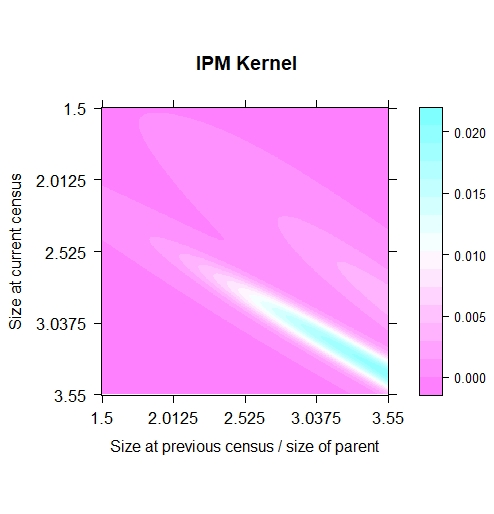
\includegraphics[scale=0.482]{ungulateEstKern.jpg}
\caption{\label{ungEstKern} Transition kernel for the \textit{Ovis aries} simulated data, using a midpoint rule with 100 points, and the estimated parameter values.}
\end{figure}

\begin{figure}
\centering
  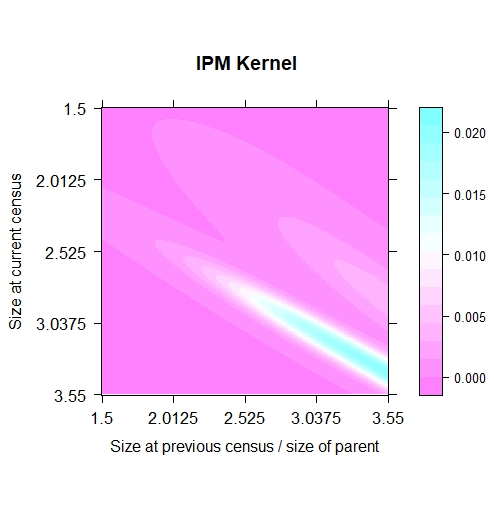
\includegraphics[scale = 0.482]{ungulateTrueKern.jpg}
  \caption{\label{ungTruKern}Transition kernel for the \textit{Ovis aries} simulated data, using a midpoint rule with 100 points, and the true parameter values.}
\end{figure}



\begin{figure}[H]
\centering
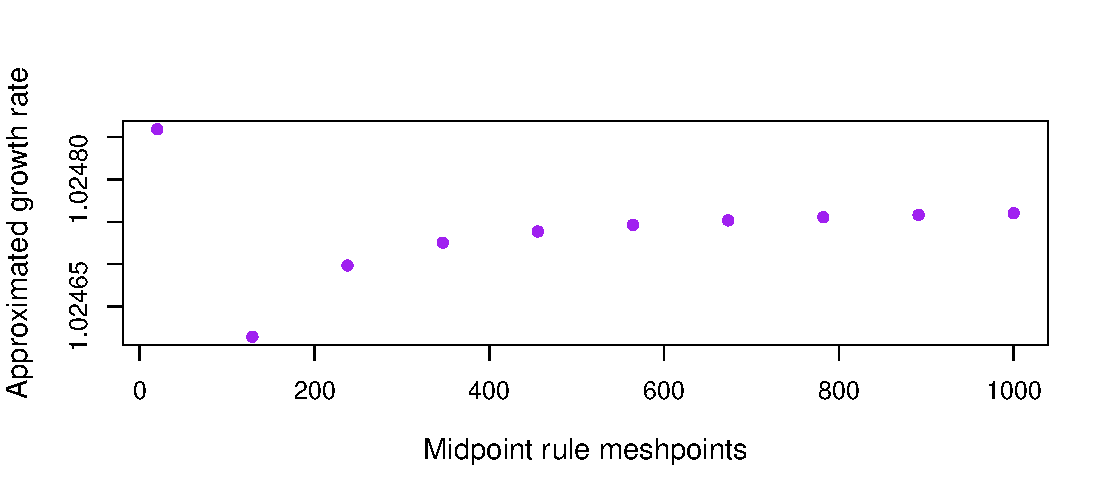
\includegraphics[scale=0.9]{growthRateMesh.pdf}
\caption{\label{grMesh}Approximated population growth rate from census to census for the \textit{Ovis aries} simulated data, using estimated parameter values and varying numbers of meshpoints for the numerical integration of the transition kernel.}
\end{figure}

\newpage
\section{State Space Model}

\subsection{Introduction}
% STATE SPACE MODEL INTRO %
In many cases, our census data include entries with unobserved individuals. This imperfect detection can lead to biases in estimations of changes in population size, and hence impede the validity of our inference \citep{gimenezRisk}. Hidden process models (where two time series are considered simultaneously: one which describes the `true' process, and one which describes the observed process) are an attractive and popular family of models to use with Integrated Population Models, due to their ability to incorporate both observation error and process variation into the analysis \citep{gimenezHPM}. A further major strength of hidden process models is their suitability to Particle Filtering and Sequential Monte Carlo. This is highly relevant for ecological modelling, as most popular Gibbs samplers (such as JAGS \citep{JAGS} or BUGS \citep{BUGS}, most commonly used by ecologists) can mix extremely poorly when the states and model parameters are highly correlated \citep{Finke}. \\

Similarly to \citet{Finke}, we define our hidden state $X_t$ to be the true population size at time $t$. However, to preserve the IPM's focus on population size structure, we extend this definition of the state such that it becomes a vector of population sizes for each size class. More precisely, $\boldsymbol{X}_t = X_t^{1:s} = (X_{t}^1, X_{t}^2, ..., X_{t}^s)$, where $s$ is the number of size classes the population has been divided into, and $X_{t}^i$ is the number of individuals that were in size class $i$ at time $t$. In the case of an IPM, $s$ is infinite, and so the decision of which grain size is most appropriate for the the data at hand lies at the discretion of the analyst. This is likely to be a compromise between the computational cost associated with including more size classes, and the minimum number of size classes which are required to achieve a discretisation grain size which is sufficient to draw meaningful inference on the demographic traits of interest. It follows that the state space $\boldsymbol{\mathcal{X}}_{1:T}$ is the set of all possible states across the whole time series. Similarly, when $Y_{t}^i$ is the random variable representing the number of detected individuals in size class $i$ at time $t$, the observation state space is denoted by $\boldsymbol{\mathcal{Y}}_{1:T}$.\\

The Hidden Process Model that we define is comprised of two parts: a model $f(\boldsymbol{X}_t \mid \boldsymbol{X}_{t-1}, \boldsymbol{\theta})$, which determines the probability of transitioning from the size distribution at time $t-1$ to the size distribution at time $t$, as well as a second component, which is the observation model $\Pr(\boldsymbol{Y}_t \mid \boldsymbol{X}_t, \boldsymbol{\theta})$, giving the probability of observing the size distribution in our data set at time $t$ when the true size distribution at time $t$ was in fact $\boldsymbol{X}_t$. In both cases, $\boldsymbol{\theta}$ is the vector containing all of the parameters which specify the IPM.\\


% STATE SPACE MODEL - SAMPLING FROM THE STATE SPACE %
\subsection{Model Specification - Sampling From the State Space}

We make no attempt to define $f(\boldsymbol{X}_t \mid \boldsymbol{X}_{t-1}, \boldsymbol{\theta})$ directly. Partly because we will later see that sampling from $f(\boldsymbol{X}_t \mid \boldsymbol{X}_{t-1}, \boldsymbol{\theta})$ is sufficient for the use of Particle Filtering, and partly because defining this state transition function via a sampling method leads more directly to an IPM-based specification. To simulate from $\boldsymbol{x}_{t-1}$ to $\boldsymbol{x}_{t}$ (realisations of $\boldsymbol{X}_{t-1}$ and $\boldsymbol{X}_{t}$), we first translate the numbers of individuals in each size class to artificial values for the size variable. Typically this is taken to be midpoint of the size class. However, we will shortly demonstrate why this needs the ability to generalise. Once the size distribution has been made continuous again, we use the IBM from section 2.1 to simulate the trajectory of the population forwards till the next census, given $\boldsymbol{\theta}$, and then we convert the continuous size distribution back to the number of individuals present in each size class.\\

\begin{figure}[H]
\centering
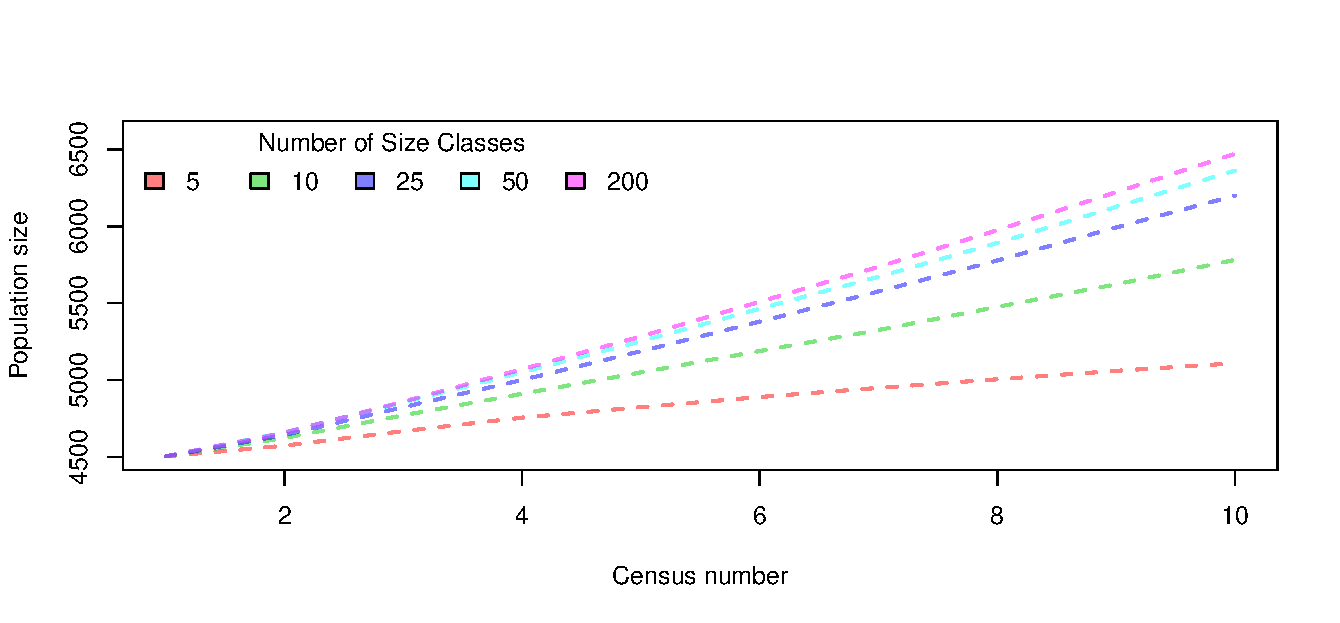
\includegraphics[scale=0.75]{sizeClasses.pdf}
\caption{\label{sizeClasses}Mean simulated population size trajectory for 10 timesteps of simulated \textit{Ovis aries} data, using the State Space Model sampler. 100 simulated trajectories were generated for each number of size classes, with a starting size counts distribution sampled multinomially, to resemble the stable size distribution of the IBM \textit{Ovis aries} data.}
\end{figure}

We can use this method to project individuals forwards for an arbitrary number of time steps, simply by converting the size class counts to a continuous size distribution at the start of each time step, and back to a discrete set of counts at the end of each time step. Using this method of simulation works well, but introduces some idiosyncrasies. Overlaying simulated trajectories from the state space sampler with varying numbers of size classes leads to figure \ref{sizeClasses}. We can clearly observe that increasing the number of size classes leads to significant increases in the population size. In fact, this is because for the parameter values we use to simulate the \textit{Ovis aries} data, size is positively correlated with survival and reproductive probability. Thus any individual that grows enough to cross a size class boundary from one census to the next, no matter by how small a margin, gets its survival probability and reproductive probability boosted to a higher value when it finds its size being estimated as being halfway through the size class. Randomly dispersing individuals throughout the size class uniformly does not correct the problem, as the expected value for the size of the individual is still higher than it should be. \\

\begin{figure}[H]
\centering
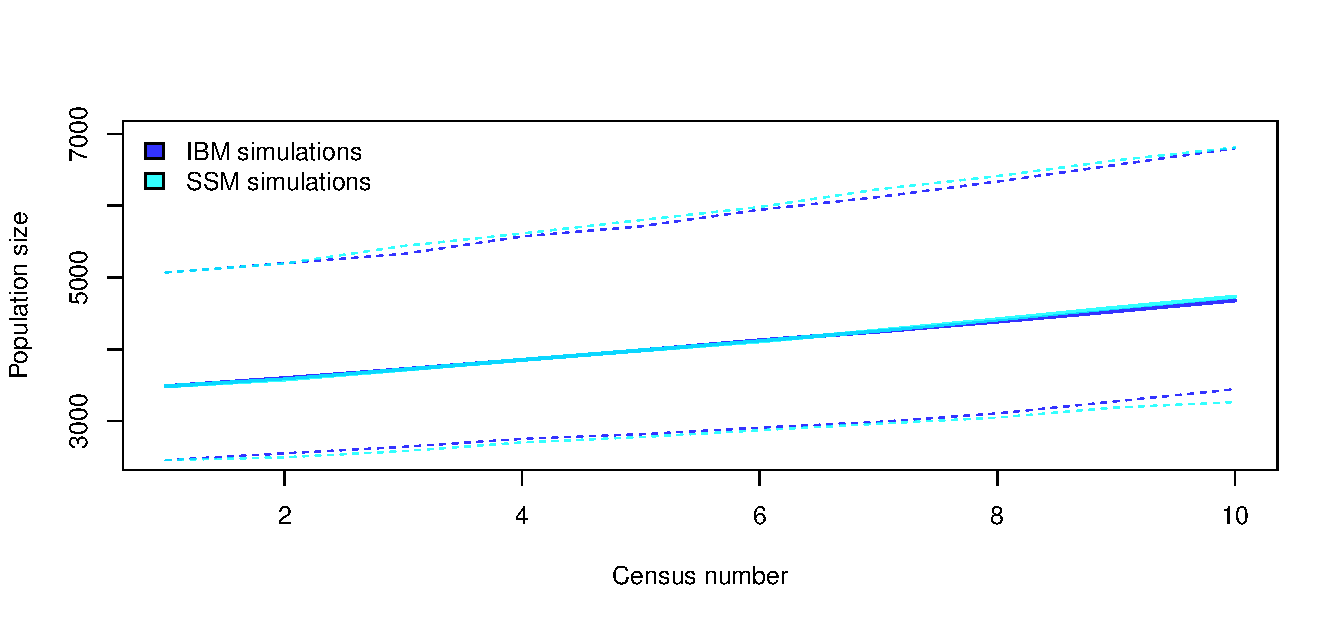
\includegraphics[scale=0.75]{shiftCorrect.pdf}
\caption{\label{correctShift}Lower 2.5\%, mean, and upper 2.5\% population size trajectory for simulated \textit{Ovis aries} data, from 50 simulated trajectories. For the State Space Model simulations, a grain size of 20 size classes was used, with size classes of even range. A `shift' value of 0.445 was used.}
\end{figure}

\begin{figure}[H]
\centering
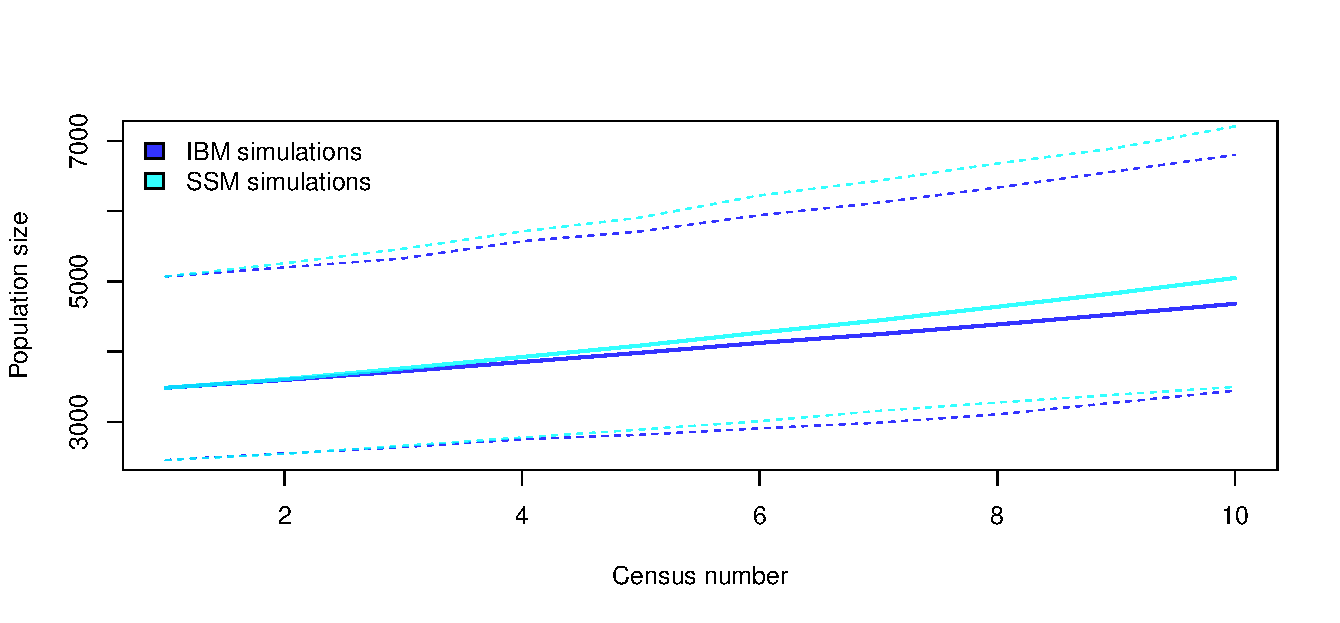
\includegraphics[scale=0.75]{shiftIncorrect.pdf}
\caption{\label{incorrectShift}Lower 2.5\%, mean, and upper 2.5\% population size trajectory for simulated \textit{Ovis aries} data, from 50 simulated trajectories. For the State Space Model simulations, a grain size of 20 size classes was used, with size classes of even range. A `shift' value of 0.5 was used.}
\end{figure}

The solution we propose is to shift the assumed size of the individual from the midpoint of the interval to some other value between 0 and 1. This `shift' is easy to figure out through simulation when dealing with known parameter values, but becomes another unknown parameter when fitting models to real data. This can be visualised using figures \ref{correctShift} and \ref{incorrectShift}. The effect isn't drastic when simulating for only 10 time steps, but as population sizes tend to increase exponentially, even a small deviation in the correct value of `shift' can lead to simulated population sizes which are orders of magnitude off of the correct value, by only an extra 10 or 20 time steps. Since the IBM simulation is very sensitive to the initial starting distribution, and often requires some `burn in' to reflect exact properties of the formulated IPM, we typically run the IBM simulation for more time steps than we require, and only use the final few generated censuses. We then use the population size of the IBM data and its empirical size distribution at our `first' census to generate the initial conditions for the State Space Model sampler, to ensure comparable setups. This process is also applicable to figure \ref{sizeClasses}.\\

\subsection{Model Specification - Our Observation Model}
%Model Specification - Our Observation Model%

In this section we seek to specify some options for the observation model $\Pr(\boldsymbol{Y}_t|\boldsymbol{X}_t)$, the probability of the observed size counts distribution at time $t$, given the true size counts distribution at time $t$. The first model which we consider only uses the total size of the population at each time point. The size of the population we observe is modelled to be the result of a binomial distribution where each animal is detected with constant probability (although this could easily be modified to allow detection probability to be a function of animal size, for example). This gives us:

\begin{equation}
    \Pr(\boldsymbol{Y}_t|\boldsymbol{X}_t, p) = {N_{\boldsymbol{X}_t} \choose N_{\boldsymbol{Y}_t}} p^{N_{\boldsymbol{Y}_t}}(1-p)^{N_{\boldsymbol{X}_t} - N_{\boldsymbol{Y}_t}}
\end{equation}

Where $N_{\boldsymbol{X}_t}$ is the total true population size at time $t$, and $N_{\boldsymbol{Y}_t}$ is the observed population size at time $t$. $p$ is the independent probability of detection for each individual. Whilst this model is very rudimentary, and uninformative on the shape of the size distribution itself, it can leverage useful analysis on the growth rate of populations of interest, when other observation models lead to computation which becomes too taxing. This observation model facilitates this by giving the same answer independently of the number of size classes being used in the analysis, whereas other models which consider size classes individually tend to produce smaller and smaller probabilities for the same data, as the number of size classes increases. This is especially true of any model which considers the count in each size class to be independent of the count in all others - leading to the product of many probabilities - which can quickly lead to underflow problems when many size classes are involved. \\

Some examples of observation models for population trait-structured count data which are found in the literature are: Normally distributed counts for each group \citep{Newman, KingBayesianPopEco}, the binomial model for total population size (as in equation 9) \citep{DailMadsen, Royle}, log-normal counts \citep{King2008}, and negative binomial counts \citep{Finke}. Log-normal and normal observation models are problematic in that they both assume counts follow a continuous distribution, with the normal distribution having the additional concerning assumption that observation errors are independent of scale \citep{Finke}. Binomial models which work out the probability of observed counts per size class (as opposed to for the whole population) are problematic for reasons which are discussed in a following section, and so aren't considered here. The negative binomial offers an attractive alternative, due to its ability to account for over-dispersion, and so we consider a modification of the model proposed by \citet{Finke}, such that $Y_t^i$, the number of individuals in size class $i$ at time $t$ is given by:

\begin{equation}
    Y_t^i \sim \text{NB}\left(\frac{\kappa}{1-\kappa}X_t^i, \kappa\right)
\end{equation}

This model assumes that the count in each size class is independent of the count in all other size classes, which introduces some unfortunate but necessary lack of realism to the modelling of the biological process. We propose another, stricter observation model, which aims to leverage as much information as possible on not only the size of the population, but specifically, the shape of its size distribution compared to that of the true state $\boldsymbol{X}_t$. This model is an extension of equation (9) in the sense that we still begin by modelling the total number of detected individuals binomially, assuming that each individual has an independent detection probability. The extension involves introducing the assumption that the observed counts across size classes follow a multinomial distribution, with the probability of belonging to any given size class being proportional to the fraction of the population in $\boldsymbol{X}_t$ that finds itself in the same size class. By combining these two elements together, we hope to gain information both on detectability of individuals, but also to guide the posterior towards sets of parameters that imply IPM formulations where simulated size distribution trajectories are as close as possible to our observed ones. Unfortunately, whilst intuitive in a statistical sense, this model struggles to relate to any meaningful real-world interpretation of the data-collection process, as it largely implies the possibility that detected individuals' sizes are mis-recorded, such that an individual may appear in a size class different to its true value. This observation model has density:

\begin{equation}
    \Pr\left(\boldsymbol{Y}_t\mid\boldsymbol{X}_t, p\right) =  {N_{\boldsymbol{X}_t} \choose N_{\boldsymbol{Y}_t}} p^{N_{\boldsymbol{Y}_t}}(1-p)^{N_{\boldsymbol{X}_t} - N_{\boldsymbol{Y}_t}}\frac{N_{\boldsymbol{Y}_t}}{Y_t^1!\cdots Y_t^s!}\rho_{t, 1}^{Y_t^1}\cdots\rho_{t, s}^{Y_t^s}
\end{equation}

Where $N_{\boldsymbol{X}_t}$ and $N_{\boldsymbol{Y}_t}$ are as before, $p$ is still the probability of detection for each individual, $Y_t^i$ is the count of individuals in size class $i$ at time $t$ and $\rho_{t, i} = \frac{X_t^i}{\sum_{i=1}^s X_t^i}$. $s$ is simply the total number of size classes that the population has been divided into. \\

The final observation model we propose attempts to still leverage information on the distribution of sizes, but in a marginally less restrictive way compared to the multinomial model. This hopefully acts as a compromise between the basic total population size model, and the multinomial model, which can be difficult to fit. Our model assumes that the observed count in each size class is Poisson distributed around the true number of individuals present in the size class, independently of the counts in all other size classes. This model is inspired by the Poisson distribution's natural suitability to count data, as well as allowing for heteroscedasticity, whereby larger true population counts lead to a higher variance in observed counts. It has the following density, allowing it to also account for detection probability:

\begin{equation}
     \Pr\left(\boldsymbol{Y}_t\mid\boldsymbol{X}_t, p\right) =  \prod_{i=1}^s \left(X_t^i\cdot p\right)^{Y_t^i}\cdot\exp{\left(-X_t^i\cdot p\right)}\left[Y_t^i!\right]^{-1}
\end{equation}

\subsection{Model Specification - Our Initial State Model}
%Model Specification - Our Initial State Model%

The most naive choice for an initial size distribution consists of stating that the probability an individual finds itself in a given size class is equal for all size classes, making the size distribution uniform. This is very easy to compute, and removes any potentially difficult prior elicitation, but is likely to lead to poor inference, as a handful of the observation models outlined in the previous section are extremely sensitive to differences in the true and observed size count distributions. An attractive alternative, when plenty of other data is available, is to assume the initial distribution is multinomial, using the abundance of previous data to estimate the probability of being in a given size class. This approach works very well in cases where the data are simulated, as we can generate an arbitrarily large set of additional data from which to form our prior knowledge, but the model is too inflexible to be used when modelling real-world data. A solution then, is to use the negative binomial for each size class, as \citet{Finke} do, or a Poisson model similar to equation (12). If very little information is available to elicit initial size distributions from experts or previous data, initial distributions which are more disperse should be favoured, to allow simulated particles to have a greater chance of producing true population size count vectors which lead to our data being likely. Note that this does not necessarily favour using flat initial distributions, such as the uniform, but rather using an initial distribution where the true count in each size class is more variable.\\

If initial population size is unknown - as it often is when detection is imperfect - it may be worth incorporating a Poisson, normal, or negative binomial initial total population size. In this way, the initial distribution would be simulated in a two step process, first determining the size of the population, and then the distribution of counts amongst the size classes. This approach reduces bias in the estimate of detection probability, by allowing us to describe our uncertainty of the initial population size with hyper-parameters. 

\subsection{Particle Markov Chain Monte Carlo}
% PARTICLE MCMC %
Since the likelihood implied by our model specification is intractable, and difficult to define analytically, we make use of particle filtering to make unbiased estimates of its true value, for a given set of observations, and a set of parameter values, $\boldsymbol{\theta}$. We propose the use of algorithm \ref{pfAlg1} below to achieve this. It should be noted that in the below algorithms, $\boldsymbol{x}^{i}_{t}$ refers to the $i^{\text{th}}$ simulation of the realised state vector $\boldsymbol{x}_t$. This shouldn't be confused with $x^i_t$, which would give the count of individuals in the $i^{\text{th}}$ size class of the realised state vector of true population size distribution. Following a similar principal, $\boldsymbol{x}_t^{1:N}$ is the collection of all $N$ simulated realisations of the true size distribution $\boldsymbol{x}_t$.

\begin{algorithm}
\caption{\label{pfAlg1} Particle Filter for estimating $\Pr(\boldsymbol{Y}_{1:T}, \boldsymbol{X}_{1:T}| \boldsymbol{\theta})$}
\begin{algorithmic}[1]
\begin{spacing}{1.8}
\STATE $\text{Set} \ N \  \text{to be the number of particles used to produce the estimate}$
\STATE $\text{Sample} \ \boldsymbol{x}_1^{i} \sim \mu(\boldsymbol{X}_1) \ \text{independently from the initial distribution} \  \forall \ i \in 1:N $
\STATE $\text{Calculate} \ w^i_1 = \Pr(\boldsymbol{y}^i_1 | \boldsymbol{x}_1^i, \boldsymbol{\theta})\  \forall \ i \in 1:N$
\FOR{$t \in 2:T$}
       \STATE $\text{Sample} \ \boldsymbol{\tilde{x}}_{t-1}^{i} \ \text{from}\ \ \boldsymbol{x}_{t-1}^{1:N} \ \text{with probability} \  w_{t-1}^{i}{\left[\sum_{i=1}^N{w_{t-1}^i}\right]}^{-1} \  \forall \ i \in 1:N$
       \STATE $\text{Generate} \ \boldsymbol{x}_t^{i} \sim f(\boldsymbol{x}_t^{i} | \boldsymbol{\tilde{x}}_{t-1}^{i}, \boldsymbol{\theta}) \ \text{independently} \  \forall \ i \in 1:N $
       \STATE $\text{Calculate} \ w^i_t = \Pr(\boldsymbol{y}^i_t | \boldsymbol{x}_t^i)\  \forall \ i \in 1:N$
\ENDFOR
\RETURN $\prod_{t=1}^T \left\{ \frac{1}{N} \sum_{i=1}^N w_t^i\right\}$
\end{spacing}
\end{algorithmic}
\end{algorithm}


With algorithm \ref{pfAlg1}, we use the transition function $f(\boldsymbol{X}_t \mid \boldsymbol{X}_{t-1}, \boldsymbol{\theta})$ to generate proposed values for the true states given the parameters, using an IBM based approach to simulate from the IPM. Given these, we can perform an importance sampling estimate of the likelihood via the observation model $\Pr(\boldsymbol{Y}_t | \boldsymbol{X}_t)$. Line 9 gives us a Del Moral \citep{DelMoral} unbiased estimate for the likelihood. Algorithm \ref{pfAlg1} is a basic bootstrap particle filter \citep{BootstrapPF} outlined in \citet{Finke}. The bootstrap particle filter is preferred for our use case due to its use of resampling at every time step to reduce particle depletion. The use of the prior kernel $f(\boldsymbol{X}_t \mid \boldsymbol{X}_{t-1})$ as the importance distribution leads to the importance weights depending only the likelihood of the observation, and not also on previous weights \citep{Overview}. The resampling step thus improves particle depletion at the cost of Monte Carlo Variance \citep{Overview}, by replacing particles with low weights with particles that have relatively much higher weights. Whilst resampling introduces dependence between the particle trajectories, which negates standard importance sampling convergence results \citep{Doucet}, the convergence of particle Markov Chain Monte Carlo methods has been established by \citet{Andrieu}.\\




Despite the resampling stage at every time step, we notice that in practice, particle depletion still remains a large issue. With many observation models, some sampled trajectories lead to the likelihood of the observation being orders of magnitude higher than others. These large differences typically lead to numerical underflow, leading to a consistent decay of particle weights over time. In many cases, the decay is so severe that the particle filter given by algorithm \ref{pfAlg1} fails to even progress to a second time step. A remedy to this problem is working on the log scale. Further to this, \citet{Overview} make reference to calculating normalised weights by removing the largest weight at a given time step from all others at the same time step. This facilitates the calculation of the larger weights, making underflow errors less drastic. Underflow may well still occur for the smaller weights as they tend to be calculated as having value 0, in most cases their size is so small compared to larger weights that this difference is negligible. This approach, referred to as the `log-sum-exp trick' and implemented concisely in the RMFSB package in R \citep{RMFSB}, combined with algorithm \ref{pfAlg1}, served as the inspiration for algorithm \ref{pfAlg2} above - The version of the particle filter that we use throughout this dissertation.\\

\begin{algorithm}[H]
\caption{\label{pfAlg2} Particle Filter for estimating $\log\Pr(\boldsymbol{Y}_{1:T}, \boldsymbol{X}_{1:T}| \boldsymbol{\theta})$}
\begin{algorithmic}[1]
\begin{spacing}{1.8}
%1
\STATE $\text{Set} \ N \  \text{to be the number of particles used to produce the estimate}$
%2
\STATE $\text{Set} \  LL=0 \ \text{to be the current value of the log likelihood}$
%3
\STATE $\text{Sample} \ \boldsymbol{x}_1^{i} \sim \mu(\boldsymbol{X}_1) \ \text{independently from the initial distribution} \  \forall \ i \in 1:N $
%4
\STATE $\text{Calculate} \ \log{w^i_1} = \log{\Pr(\boldsymbol{y}^i_1 | \boldsymbol{x}_1^i)}\  \forall \ i \in 1:N$
%5
\STATE $\text{Calculate} \ r^i_1 = \log{w_1^i} - \max{(\log{w_1^{1:N}})} \  \forall \ i \in 1:N $
%6
\STATE $\text{Calculate} \ s_1^i = \exp{(r_1^i)} \  \forall \ i \in 1:N $
%7
\STATE $LL = LL + \max{(\log{w_1^{1:N}})} + \log{(\frac{1}{N}\sum_{i=1}^N s_1^i)}$
%8
\FOR{$t \in 2:T$}
        %9
       \STATE $\text{Sample} \ \boldsymbol{\tilde{x}}_{t-1}^{i} \ \text{from}\ \ \boldsymbol{x}_{t-1}^{1:N} \ \text{with probability} \  s_{t-1}^{i}{\left[\sum_{i=1}^N{s_{t-1}^i}\right]}^{-1} \  \forall \ i \in 1:N$
       %10
       \STATE $\text{Generate} \ \boldsymbol{x}_t^{i} \sim f(\boldsymbol{x}_t^{i} | \boldsymbol{\tilde{x}}_{t-1}^{i}, \boldsymbol{\theta}) \ \text{independently} \  \forall \ i \in 1:N $
       %11
       \STATE $\text{Calculate} \ \log{w^i_t} = \log{\Pr(\boldsymbol{y}^i_t} | \boldsymbol{x}_t^i)\  \forall \ i \in 1:N$
       %12
       \STATE $\text{Calculate} \ r^i_t = \log{w_t^i} - \max{(\log{w_t^{1:N}})} \  \forall \ i \in 1:N $
       %13
       \STATE $\text{Calculate} \ s_t^i = \exp{(r_t^i)} \  \forall \ i \in 1:N $
       %14
       \STATE $LL = LL + \max{(\log{w_t^{1:N}})} + \log{(\frac{1}{N}\sum_{i=1}^N s_t^i)}$
\ENDFOR
\RETURN $LL$
\end{spacing}
\end{algorithmic}
\end{algorithm}

This algorithm is far more robust to numerical errors, and is appropriate given our desire to explore the log posterior space using Markov Chain Monte Carlo, for numerical stability. Unfortunately however, when certain observation models produced probabilities of 0 for a certain observation given a sampled state, particle depletion remained prominent. This situation is unfortunately very common, especially when considering any observation model which assumes that the number of detected animals in each size class must necessarily be smaller than the true number of animals present in that size class (which is an extremely reasonable assumption). In this situation, we require only a single simulated size class to contain fewer individuals than our observed count, for the probability of the whole vector of observed counts given the simulated counts to be 0. This lead to some careful consideration of which observation models would be appropriate given the computational burden of achieving higher effective sample sizes when particle depletion is significant (which will be explored further in the next section), but also lead to the implementation of another numerical trick to help stability. In lines 5 and 12 of algorithm \ref{pfAlg2}, before the residual log weights are exponentiated, we replace any values of the R object `-Inf' with -300. This maps probabilities of 0 to a probability of $\exp(-300)\approx 5\cdot 10^{-131}$. This value can be modified if required, but was found to strike a good balance between increasing numeric stability, and retaining the ability to distinguish between `poor' and `extremely poor' choices of parameters, which lead to log likelihood values which are negative and large in magnitude.\\

\begin{algorithm}[H]
\caption{\label{pmcmcAlg} Particle MCMC for obtaining samples from the posterior distribution}
\begin{algorithmic}[1]
\begin{spacing}{2}
\REQUIRE $\boldsymbol{\theta}^0 \ \text{; the initial proposed model parameters}$
\STATE $\text{Set} \ N \ \text{to be the number of desired samples}$
\FOR{$i \in 1:N$}
    \STATE $\text{Propose} \ \boldsymbol{\theta}^{*} $
    \STATE $\text{Use algorithm \ref{pfAlg2} to estimate} \
    \Pr(\boldsymbol{Y}_{1:T} , \boldsymbol{X}_{1:T} | \boldsymbol{\theta}^{*})$
    \STATE Calculate \begin{Large}$\ \alpha = \frac{\pi(\boldsymbol{\theta}^{*})}{\pi(\boldsymbol{\theta}^{i-1})}\frac{g\left(\boldsymbol{\theta}^{i-1}|\boldsymbol{\theta}^{*}\right)}{g\left(\boldsymbol{\theta}^{*}|\boldsymbol{\theta}^{i-1}\right)}$\end{Large}
    \STATE With probability $\alpha$ set $\boldsymbol{\theta}^{t} = \boldsymbol{\theta}^{*}$
    \STATE Otherwise set $\boldsymbol{\theta}^{t} = \boldsymbol{\theta}^{t-1} $
\ENDFOR
\RETURN $\boldsymbol{\theta}^{1:N}$
\end{spacing}
\end{algorithmic}
\end{algorithm}
% pMCMC

Now that algorithm \ref{pfAlg2} establishes a method for drawing samples from the log likelihood, we specify the Particle Markov Chain Monte Carlo (PMCMC) algorithm which we use to draw samples from the posterior distribution for our analyses. This sampler is a standard Metropolis-Hastings algorithm \citep{Hastings} with an adaptive random walk Gaussian proposal. If desired, the user can supply a function (typically, the sample covariance function) which uses the previously obtained samples to update the covariance structure of the proposal distribution. This adaptation occurs at 25\% and 50\% of the way through the algorithm's iterations, and the vast majority of the time, these first 50\% of the samples are discarded as part of the chain's `burn in' phase. Algorithm \ref{pmcmcAlg} above, transcribed from \citet{Finke} gives a slight simplification of the PMCMC algorithm we use, by ignoring the adaptation steps. A further advantage of using particle MCMC is the lack of tuning parameters, aside from the covariance structure of the proposal distribution, which can typically be improved by either using more samples to allow the adaptation process to work with more information, or to start a new chain using the covariance structure of the samples drawn from a previous chain.\\

\newpage
\section{Revisiting \textit{Ovis aries}}
% OVIS ARIES SMC %

\subsection{Simulating our Data}
% SIMULATING THE DATA %
Having introduced the Integral Projection Model, the traditional methodology for solving the vital rate parameters in a piecemeal fashion, and defined a state space model specification which allows us to conduct the analysis in a Bayesian setting, we wish to undertake an analysis of the simulated \textit{Ovis aries} data, to showcase the use of the proposed methodology. Unfortunately, despite being able to run particle MCMC chains in parallel (coarse grain, on multiple cores of a CPU) and including the use of custom C++ code to speed up the calculation, there is little to be done about the inherent computationally slow nature of needing to require the IBM to generate true state data for the particle filter. The IBM's speed is largely capped by that of the vital rate functions we specify, which are lightweight wrappers for base R samplers for binomial and normal distributions, which use C or Fortran code already. To help alleviate some of the computational pressures that arise from this type of analysis, we propose a short, 6 census time series, attempting to strike a balance between our available computing power, and our desire to be data-rich enough to gain meaningful insight on likely values of our parameters, \textit{a posteriori}.\\

Even when specifying the starting size distribution to be very close to that of the stable size distribution, data generated via the IBM can take a few censuses to start to behave closely to what we expect. Because of this, we choose to generate our sample data once again by simulating more time steps than we require, and taking the final 6 censuses of this simulation. Because Section 2.3 also revealed that truncation of the growth and offspring size distributions made minimal difference to estimated parameter values for the \textit{Ovis aries} data, we opt to use the non-truncated normal distribution specification for these vital rates, to avoid the negative impact a rejection sampling algorithm would have on our overall computation time. Avoiding this truncation also has the added benefit of leading to a far easier implementation and specification, as the functions which sample from the growth and offspring size distributions do not need to be passed additional parameters (the limits of the truncation). \\

We choose to use size classes with an even width. Since the size of the \textit{Ovis aries} data is measured on the log-scale, we could specify different breakpoints to ensure the size classes have even width on the linear scale instead. In practice, this leads to most of our classes remaining empty, due to the relatively skewed stable size distribution that arises when simulating these data. This is a waste of computational resources, as increasing the number of size classes makes the algorithm converge less easily by increasing complexity, and also has a tendency to drastically increase the Monte Carlo Variance of the particle filter, which furthers the problem. For these reasons, using only five size classes which are of even width on the log-scale is preferred. As is visible from figure \ref{simmedDataAll} and table \ref{ungData}, even with as few as five even width size classes, we have a size class whose counts are close to null for the length of the study. In light of this, we collapse the size classes for the two smallest groups of sizes together, to avoid unnecessary computation - leading to a four size class survey. Table \ref{UngData} then gives us the final table of counts which were used in the analysis. \\

\begin{figure}[H]
\centering
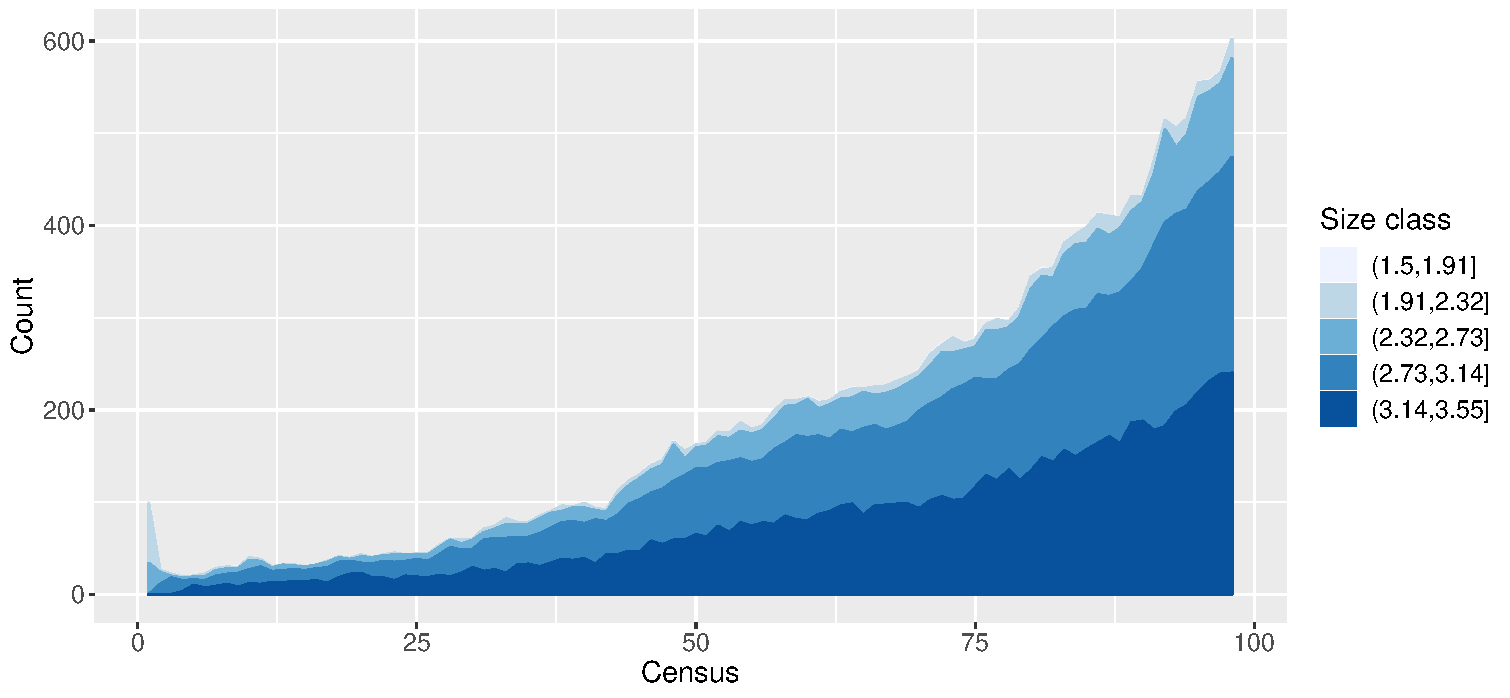
\includegraphics[scale=0.68]{simmedDataAllCensuses.pdf}
\caption{\label{simmedDataAll}Population size for the \textit{Ovis aries} data simulated from the IBM for the PMCMC case study, with counts broken down by size class for each census.}
\end{figure}

\vspace{0.5cm}

\begin{table}[ht]
\centering
\begin{tabular}{ccccccc}
  \hline
 & census 1 & census 2 & census 3 & census 4 & census 5 & census 6 \\ 
  \hline
  size class = (1.50, 1.91] & 0 & 0 & 1 & 1 & 1 & 2 \\ 
  size class = (1.91, 2.32] & 21 & 17 & 16 & 11 & 12 & 21 \\ 
  size class = (2.32, 2.73] & 72 & 82 & 102 & 98 & 96 & 107 \\ 
  size class = (2.73, 3.14] & 214 & 212 & 218 & 216 & 219 & 234 \\ 
  size class = (3.14, 3.55] & 198 & 205 & 219 & 231 & 239 & 240 \\ 
   \hline
\end{tabular}
\caption{\label{ungData}Size class counts for the last 6 censuses of the \textit{Ovis aries} data which were simulated for the particle MCMC case study.}
\end{table}

\vspace{0.5cm}

\begin{table}[ht]
\centering
\begin{tabular}{rrrrrrr}
  \hline
 & census 1 & census 2 & census 3 & census 4 & census 5 & census 6 \\ 
  \hline
  size class = (1.50, 2.32] & 21 & 17 & 17 & 12 & 13 & 23 \\ 
  size class = (2.32, 2.73] & 72 & 82 & 102 & 98 & 96 & 107 \\ 
  size class = (2.73, 3.14] & 214 & 212 & 218 & 216 & 219 & 234 \\ 
  size class = (3.14, 3.55] & 198 & 205 & 219 & 231 & 239 & 240 \\ 
   \hline
\end{tabular}
\caption{\label{UngData}Size class counts for the last 6 censuses of the \textit{Ovis aries} data which were simulated for the particle MCMC case study, with the two smallest size classes combined.}
\end{table}

\subsection{Determining PMCMC settings}
% DETERMINING PMCMC SETTINGS %
We aim to investigate the correlation structure between variables of interest, and to compare if this indicates that the traditional piecemeal approach makes an unrealistic assumption of independence by fitting the vital rate functions separately. To avoid skewing this comparison by bringing in any \textit{a priori} information, we place uniform priors on all parameters of interest. We determine the prior population starting size distribution via simulation of the IBM. We replicate the process that generated our data to gain an idea of the average probability of belonging to each size class, and we fix the starting population size to be the same as that of our data. We run 100 replications and obtain estimated probabilities for being in each class of approximately $0.034, 0.168, 0.399, 0.399$, respectively. We do not remove any of our observations, such that the expected probability of detection is 1.

We select the observation model which considers only the total number of detected animals, since more complicated models require far higher numbers of particles to be feasible on the available hardware (Intel Core i7-6700k overclocked to 4.2 GHz, 32GB RAM), due to having larger standard deviations in their estimates of the log-likelihood. Many attempts were made to fit these different observation models, and an appropriate covariance structure for the proposal could never be found, despite the significant time commitment this represented during the project. Fitting these observation models would require a far more substantial time investment for the implementation, such that all the required libraries could be written in C, rather than the current implementation entirely in R (with only snippets of C code to optimise the most taxing functions). Access to a cluster of computers may also make these observation models more tractable, however this wouldn't provide significant aid in finding appropriate proposals or running chains till convergence, which remains the largest limitation.

As well as opting for a shorter time series, we attempt to minimise the number of particles the filter uses for each estimation of the likelihood. Since this filter is run many times over the course of the particle MCMC, any reduction in the particle set size can lead to drastic savings in overall computing time. Despite the issue of particle depletion, which can be so bad as to lead to effective sample sizes in the tens, when the number of particles are in the millions \citep{Newman}, we observe that in practice, the variance of our estimates of the likelihood can be confined within a tolerable range with particle numbers between $10^2$ and $10^3$. A quick demonstration of this, by calling the particle filter to estimate the value of the log-posterior evaluated at the true parameter values is given by figure \ref{particleNum}. A particle set size of 100 leads to a standard deviation of 8.76, which drops to 4.58 for 250 particles, and 2.20 for 500. \citet{DoucetEfficient} suggest that when the efficiency of a Metropolis-Hastings algorithm using the exact likelihood is unknown, using a particle set size which leads to a standard deviation of around 1.2 for the unbiased estimate of the log-likelihood minimises the upper bound on the total computing time required to achieve a given asymptotic variance for a particular pseudo-marginal average. Via some simulations using 10000 estimations of the value of the log-likelihood at the true parameter values for various numbers of particles used, it would appear a particle set size of around 435 achieves this standard deviation of 1.2.

The effective sample size of the particle filter for various number of particles used is given by table \ref{ESS}. In this table, we do not consider the effective sample size at the first time step as this is always equal to the number of particles the filter is using.

\begin{table}[H]
\centering
\begin{tabular}{cccccc}
  \hline
 Particles & 100 & 250 & 435 & 500 & 1000\\ 
  \hline
 Effective samples size & 2.28 & 4.45 & 7.59 & 8.70 & 17.44 \\
   \hline
\end{tabular}
\caption{\label{ESS}Estimated effective sample size of the particle filter for censuses 2 to 6 for the table \ref{UngData} count data, evaluated at the known parameter values. 500 runs of the particle filter were used to estimate the average effective sample size across the censuses.}
\end{table}

\begin{figure}[H]
\centering
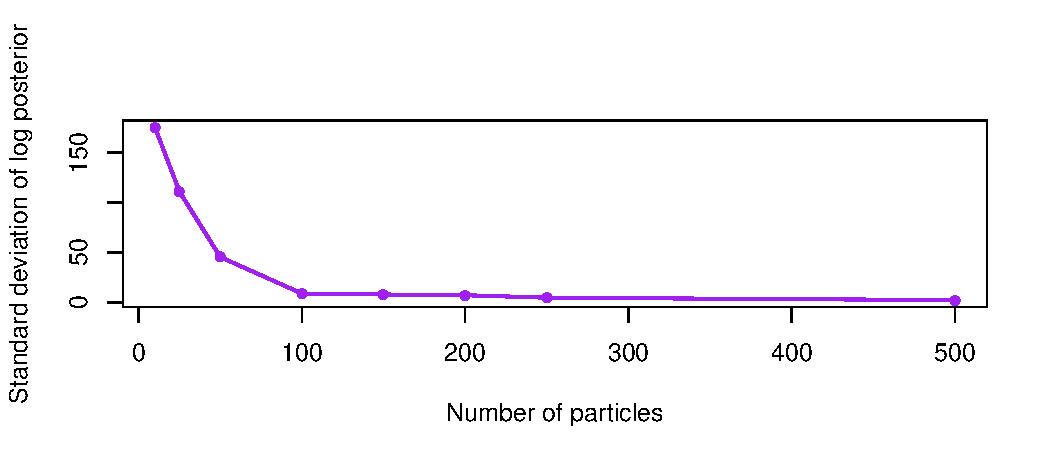
\includegraphics[scale=0.9]{particleNum.pdf}
\caption{\label{particleNum}Standard deviation of the log posterior evaluated at the known parameter values for the \textit{Ovis aries} simulated data with the table \ref{UngData} size class breakpoints. 20 Evaluations of the log posterior were used to estimate the standard deviation for each given particle set size.}
\end{figure}


To attempt to reduce the dimensionality of the problem, we would like to consider `shift' not as a random variable, but as a known value. Since the \textit{Ovis aries} data are simulated, we can use the same approach as Section 3.2 to find this value. We use the same parameter values, and the breakpoints for size classes given in table \ref{UngData}. As is illustrated in figure \ref{ungFlat50}, using the default value of $\text{`shift'} = 0.50$ only leads to a minimal upwards drift of the population size compared to IBM simulations. At only 6 time steps, this difference is almost small enough to be considered negligible. However, figure \ref{ungFlat49} shows that using a value of 0.49 is better, leading to an almost perfect overlap of the two curves at both the $6^{\text{th}}$ and $10^{\text{th}}$ time steps.

\begin{figure}[H]
\centering
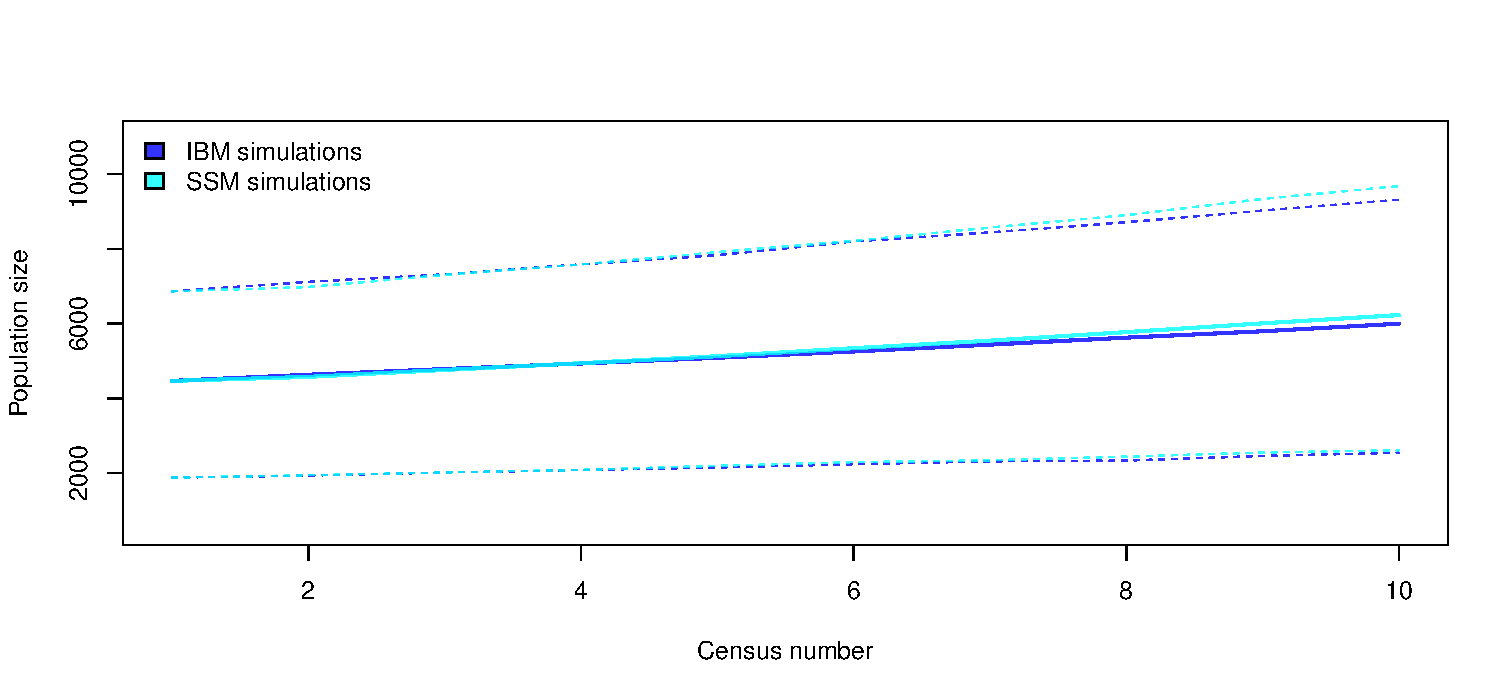
\includegraphics[scale=0.65]{ungData50.pdf}
\caption{\label{ungFlat50}Lower 2.5\%, mean, and upper 2.5\% population size trajectory for simulated \textit{Ovis aries} data, from 20 simulated trajectories. For the State Space Model simulations, the table \ref{UngData} breakpoints were used. A `shift' value of 0.50 was used.}
\end{figure}

\begin{figure}[H]
\centering
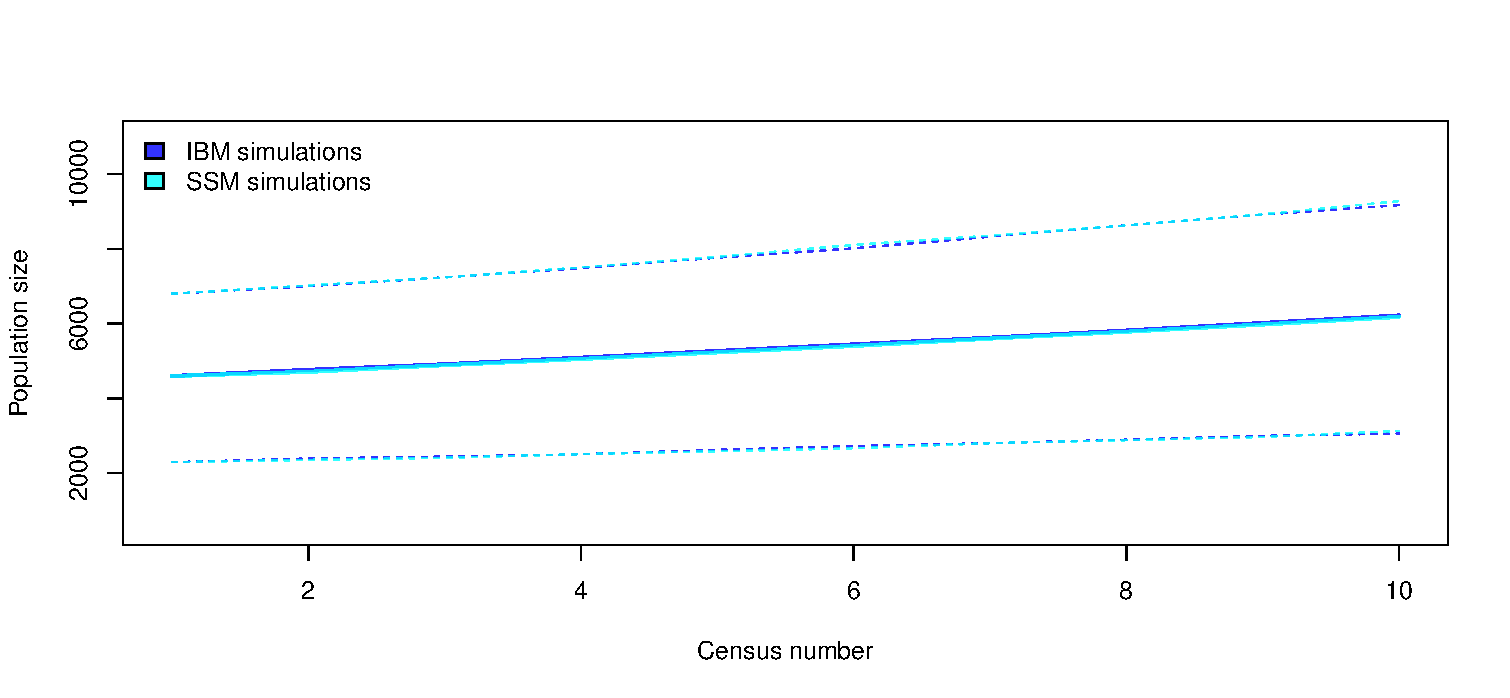
\includegraphics[scale=0.65]{ungData49.pdf}
\caption{\label{ungFlat49}Lower 2.5\%, mean, and upper 2.5\% population size trajectory for simulated \textit{Ovis aries} data, from 20 simulated trajectories. For the State Space Model simulations, the table \ref{UngData} breakpoints were used. A `shift' value of 0.49 was used.}
\end{figure}

\subsection{Running the PMCMC Chains}

A standard approach to estimating the appropriate covariance structure of a Gaussian random walk proposal distribution, is to begin with an over-dispersed isotropic proposal, which then becomes more refined as we use the covariance structure of the samples to update the proposal. This method did not lead to good convergence in the case of our setup, because typical guesses for starting standard deviations (in the order of $10^{-3}$ to $10^{1}$) generated very few accepted sets of parameters (acceptance probability ranging from $10^{-3}$ to $10^{-2}$), producing very narrow covariance structures when we used the previous samples to update the proposal covariance structure. Because of this, we tried a more sophisticated method of finding a suitable starting proposal, turning to simulated annealing to find the \textit{maximum a posteriori} (MAP) of our model. We performed 1000 iterations of this algorithm, with starting values equal to the parameter values we simulated our data from, using the R function `optim'. This function can also provide us with an estimate of the Hessian matrix of the estimates it has found, which we invert to find an estimate of the log posterior's covariance structure. In order to increase the accuracy of our estimation of the MAP, we increase the number of particles per iteration to 1000. This leads to the estimated values given in tables \ref{SANN1} and \ref{SANN2}. In practice, chains which were run with this estimated starting proposal covariance structure always produced chains with an acceptance probability which was too high for good mixing (between 0.35 and 0.5). Inspection revealed that the estimated proposal standard deviations for each parameter were in the order of $10^{-8}$ to $10^{-5}$, which is far smaller than values which had previously been considered. New scaling values were tested, until pilot chains producing 1000 samples had an acceptance ratio between 0.2 and 0.25. Using 250 particles per evaluation of the log likelihood, this lead to a starting standard deviation of $5 \cdot 10^{-5}$ for each component of the (isotropic) Gaussian proposal. \\

\begin{table}[ht]
\centering
\begin{tabular}{ccccccc}
  \hline
 & survival.i & survival.s & growth.i & growth.g & growth.sd & detection.p \\ 
  \hline
Estimated & -9.67 & 3.87 & 1.54 & 0.42 & 0.02 & 1 \\ 
  True & -9.65 & 3.77 & 1.41 & 0.56 & 0.08 & 1 \\ 
   \hline
\end{tabular}
\caption{\label{SANN1}Estimated parameter values for the `survival and growth' kernel of the IPM, based on the simulated \textit{Ovis aries} count data, using 1000 iterations of simulated annealing.}
\end{table}


\begin{table}[ht]
\centering
\begin{tabular}{cccccccc}
  \hline
 & repr.i & repr.g & litter.size & off.size.i & off.size.g & off.size.sd & child.survival.p \\ 
  \hline
Estimated & -7.29 & 2.94 & 1.09 & -0.63 & 1.33 & 0.15 & 0.74 \\ 
  True & -7.23 & 2.60 & 1.00 & 0.36 & 0.71 & 0.16 & 0.87 \\ 
   \hline
\end{tabular}
\caption{\label{SANN2}Estimated parameter values for the `offspring' kernel of the IPM, based on the simulated \textit{Ovis aries} count data, using 1000 iterations of simulated annealing.}
\end{table}

Having obtained this initial proposal distribution, we run some chains simultaneously in parallel, on different cores of the CPU, starting at the MAP found through simulated annealing. These chains then undergo several cycles of being re-run, using the covariance structure of the generated samples as a way of improving on the covariance structure of the proposal with every cycle. The next set of chains is always started at the end point of the chains in the previous set. Once trace plots of the chains indicate that the proposal is adequate, we halt this process and run a final set of chains for a larger number of samples. We ran one set of 8 chains where the particle filter uses 250 particles per evaluation of the log-likelihood, and another of 4 where the particle filter uses the 435 particles per evaluation that we deem closer to optimality. Both sets of chains seem to converge similarly well, but we choose to focus on the four chains using more particles, since these should produce more precise estimates of the growth rate of the population.

% DIAGNOSTICS %
\subsection{Results}
The final set of chains was run for 18000 iterations, with (very minor) adaptation of the proposal at sample 4500 and sample 9000. Convergence of the chains is good, as assessed via the Gelman-Rubin diagnostic \citep{GRTest} (figure \ref{GR3}), and we deem there is no need to remove part of the chain as a burn in. All diagnostic plots are available for each of the 4 chains individually, for all 13 parameters, in high resolution PDFs, in the link to supplementary materials in the appendix. For the purpose of saving space, the plots in this section only include the first two parameters. Traceplots also give a strong indication of convergence (figure \ref{trace3}). Acceptance ratios for each of the chains are 0.300, 0.300, 0.289 and 0.300 respectively, which is slightly higher than optimal. Autocorrelation in the chains doesn't die off until around a lag of around 30 (figure \ref{acf3}), and so we choose to thin the chains by a factor of 10 to remove this. This leaves us with 1800 samples per chain, and an effective sample size of 93.7, 101.9, 105.8 and 103.9, for each of the four chains respectively. The autocorrelation now dies completely at around lag 5 (supplementary materials). Tables \ref{post1} and \ref{post2} give the MAP, mean, median and 95\% credible interval for each of the parameter values. It's clear from these tables that the analysis would have benefited from making use of informative priors. For example, the litter size, which is held fixed at 1 in the simulation (and is extremely close to 1 for real populations), has been estimated as being around 5. Since parameters are updated simultaneously by the sampling algorithm, this will have biased our estimation of other parameters.

\begin{figure}[H]
\centering
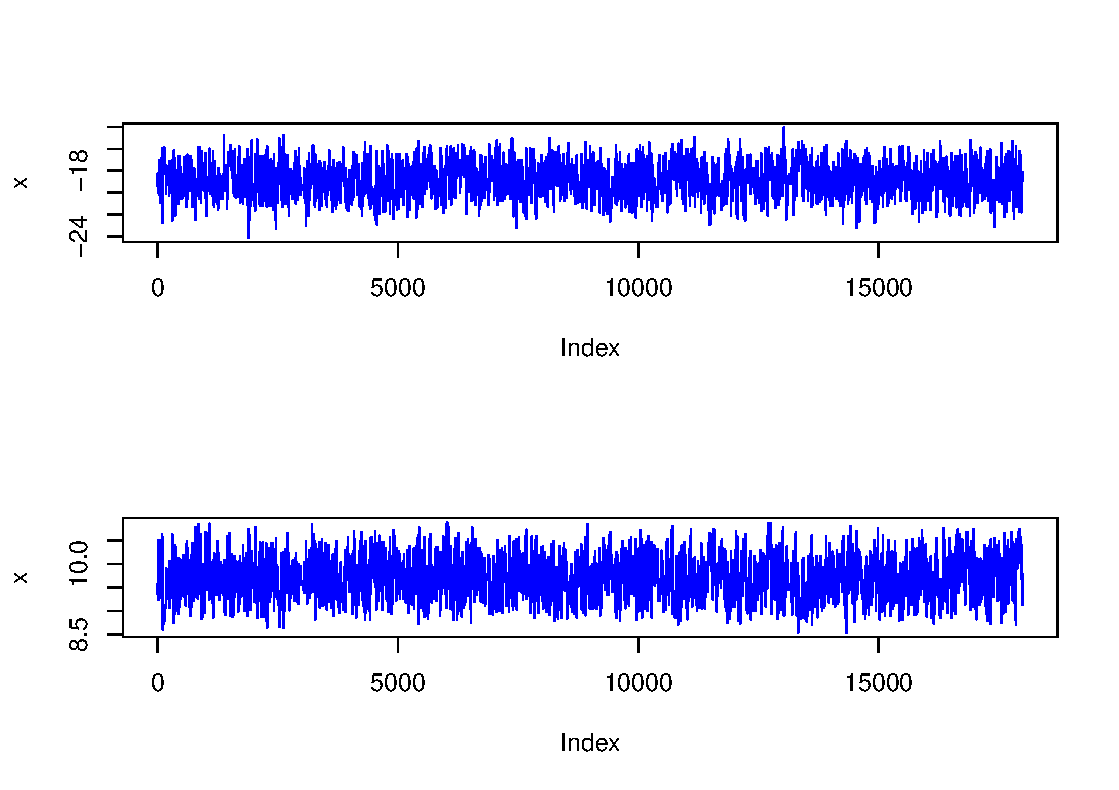
\includegraphics[scale=0.75]{chainFirst3_1.PDF}
\caption{\label{trace3}Trace plots for the first two parameters of the first chain of the \textit{Ovis aries} simulated data particle Markov Chain Monte Carlo output.}
\end{figure}

\begin{figure}[H]
\centering
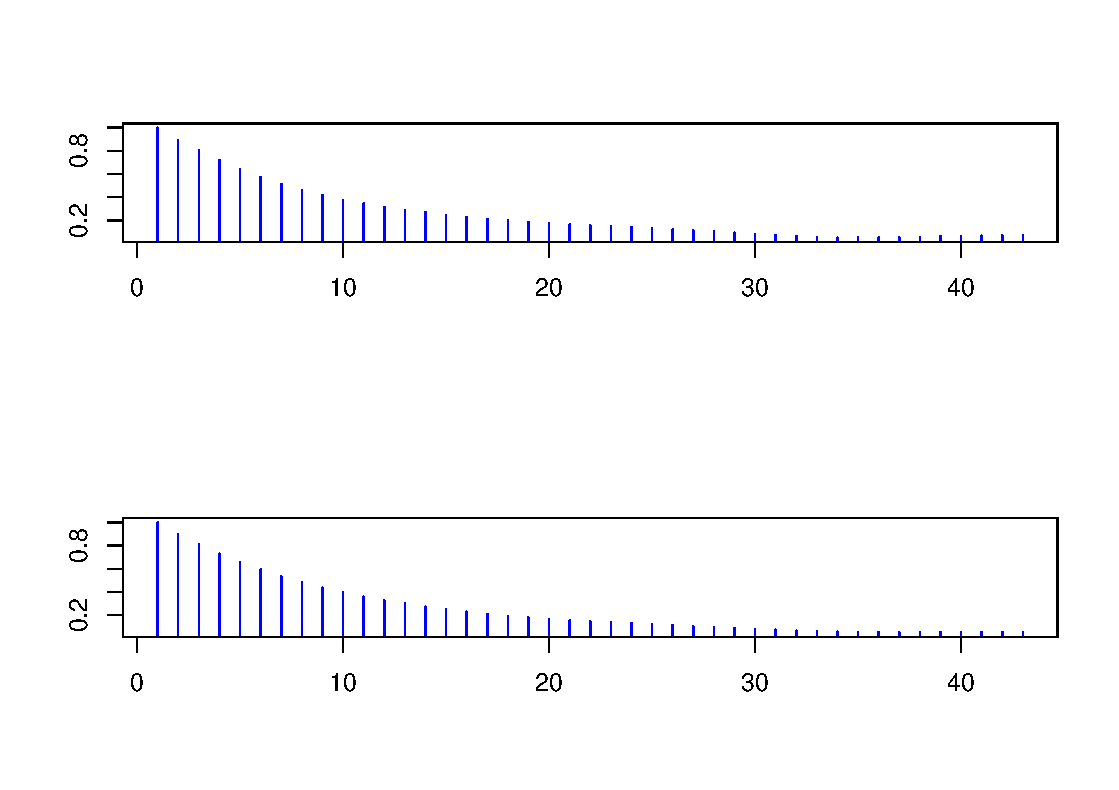
\includegraphics[scale=0.75]{chainFirst3_2.PDF}
\caption{\label{acf3}Autocorrelation plots for the first two parameters of the first chain of the \textit{Ovis aries} simulated data particle Markov Chain Monte Carlo output.}
\end{figure}

\begin{figure}[H]
\centering
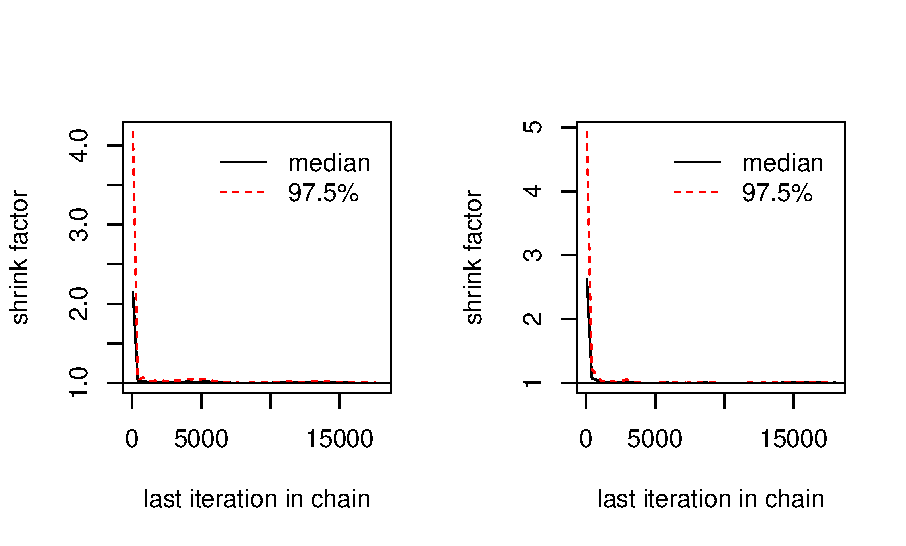
\includegraphics[scale=0.9]{GRFirst2.pdf}
\caption{\label{GR3}Gelman-Rubin convergence diagnostic plots for the first two parameters of the first chain of the \textit{Ovis aries} simulated data particle Markov Chain Monte Carlo output.}
\end{figure}

\begin{table}[ht]
\centering
\begin{tabular}{rrrrrrr}
  \hline
 & survival.i & survival.g & growth.i & growth.g & growth.sd & observation.p \\ 
  \hline
simulated & -9.65 & 3.77 & 1.41 & 0.56 & 0.08 & 1.00 \\ 
  MAP & -20.71 & 10.20 & -0.16 & 2.66 & 0.08 & 1.00 \\ 
  mean & -18.89 & 9.69 & -0.98 & 2.77 & 0.04 & 1.00 \\ 
  median & -18.86 & 9.67 & -1.46 & 2.93 & 0.01 & 1.00 \\ 
  lower & -21.78 & 8.89 & -4.30 & 0.75 & 0.00 & 1.00 \\ 
  upper & -16.04 & 10.57 & 5.80 & 3.67 & 0.31 & 1.00 \\ 
   \hline
\end{tabular}
\caption{\label{post1} Posterior parameter values for the state space model analysis of simulated \textit{Ovis aries} data, for the growth kernel of the IPM, including the boundaries of a 95\% credible interval}
\end{table}

\begin{table}[ht]
\centering
\begin{tabular}{rrrrrrrr}
  \hline
 & repr.i & repr.g & litter.size & off.size.i & off.size.g & off.size.sd & child.survival.p \\ 
  \hline
simulated & -7.23 & 2.60 & 1.00 & 0.36 & 0.71 & 0.16 & 0.87 \\ 
  MAP & -11.07 & 0.95 & 4.98 & -3.44 & -4.94 & 0.11 & 1.00 \\ 
  mean & -11.86 & 1.04 & 5.31 & -6.71 & -3.17 & 0.10 & 1.00 \\ 
  median & -11.75 & 1.05 & 4.95 & -6.80 & -3.10 & 0.10 & 1.00 \\ 
  lower & -13.82 & 0.89 & 3.40 & -11.59 & -6.08 & 0.07 & 0.97 \\ 
  upper & -10.33 & 1.18 & 9.16 & -1.58 & -0.46 & 0.13 & 1.00 \\ 
   \hline
\end{tabular}
\caption{\label{post2} Posterior parameter values for the state space model analysis of simulated \textit{Ovis aries} data, for the reproduction kernel of the IPM, including the boundaries of a 95\% credible interval}
\end{table}

It's interesting to note that the MAP we found through the PMCMC is substantially different from that obtained through simulated annealing, which may not be as adept at exploring the posterior space. Because parameter estimates differ so significantly from the simulated values, we are unable to capture the population growth rate well. The growth rate (as determined by the leading eigen value of a numerical approximation of the IPM kernel) is estimated to be 0, or very close to zero, for the MAP, and for the lower and upper bounds of a 95\% credible interval. This could highlight an issue of parameter identifiability in the model's current formulation. For example, litter size and offspring survival are extremely hard to parse apart without any direct data on proportions of children which are born but don't survive till first census. We therefore would favour an approach which allows the use of other, or previous data sets to form tight priors on these parameters such that a Bayesian analysis uncovers parameter correlation which is due to the underlying biological mechanism, as opposed to a result forced by the chosen parameterisation. With this said, a subset of the marginal posterior distributions from our analysis is given by figure \ref{partialMarg}, which shows that parameters which should not \textit{a priori} be difficult to tease apart are still highly correlated in their posterior marginal distributions, suggesting that the traditional piecemeal approach is inadequate, and motivating further exploration of a Bayesian alternative. Detailed marginal plots for all chains and all parameters are available in the supplementary material.

\begin{figure}[H]
\centering
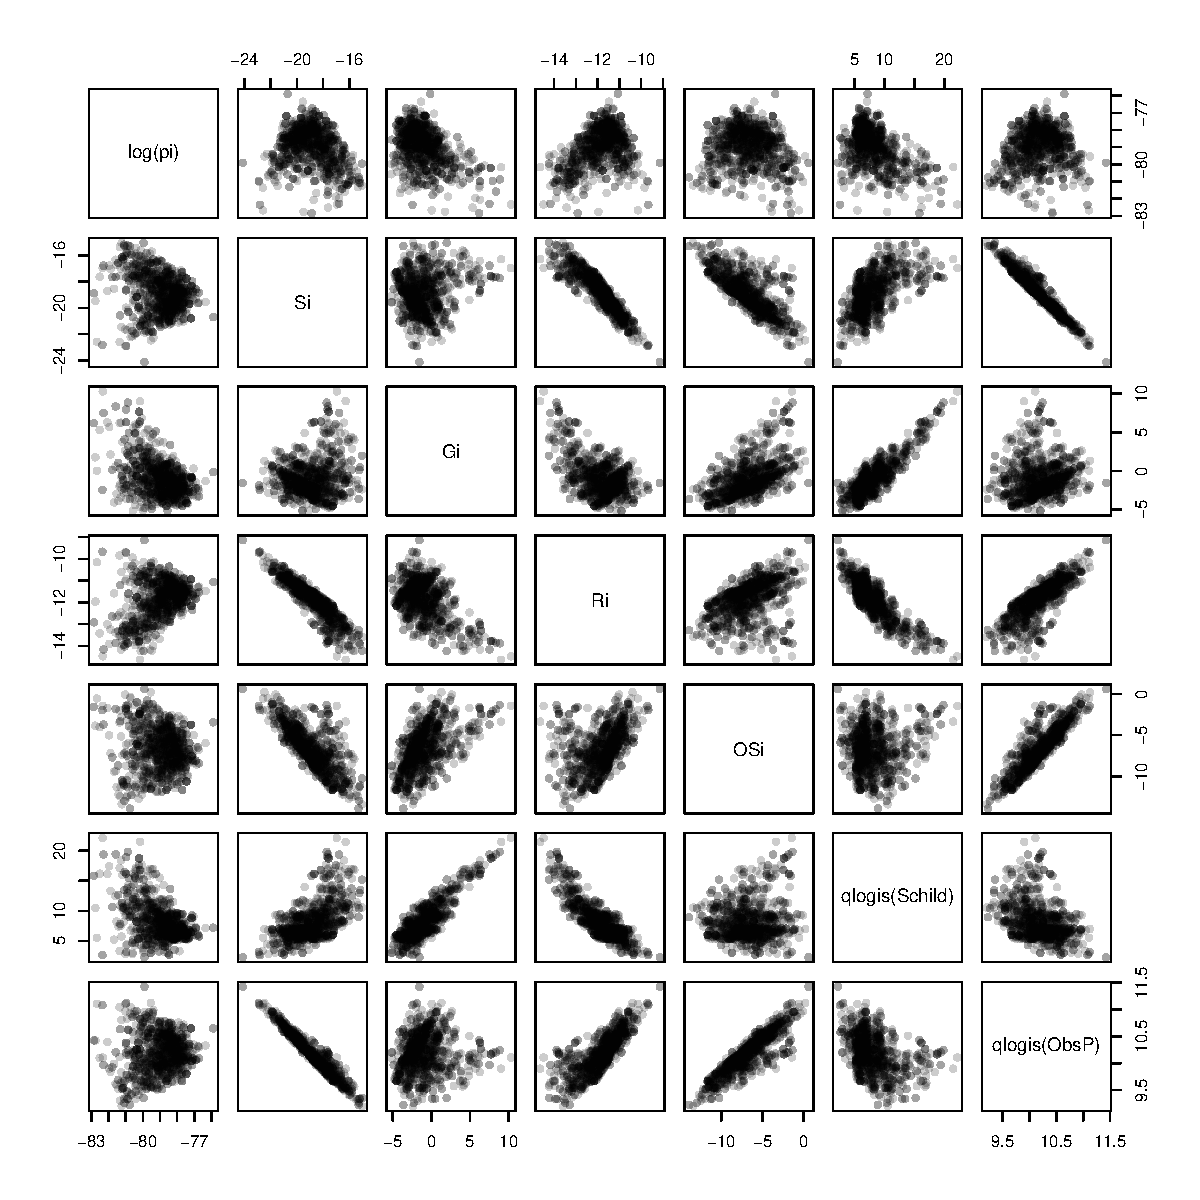
\includegraphics[scale=0.77]{chain1partialMarg.PDF}
\caption{\label{partialMarg}Conditional marginal distributions for the intercepts and probability parameters of the PMCMC analysis on simulate \textit{Ovis aries} data, for the first chain}
\end{figure}

\newpage
\section{\textit{Ovis aries}, real data}
\subsection{Data and PMCMC setup}
% DATA AND PMCMC SETUP  REAL SHEEP DATA%
We turn to a real data set for \textit{Ovis aries}, hoping to fit a state space model via particle MCMC in order to compare our results with the analysis performed by \citet{Coulson2012}. The data consist of 11 yearly surveys of the females in a population of Soay Sheep in Village Bay, St Kirta, Scotland. Almost all of the individuals in the population are detected during the yearly survey, but few (around half) are caught and weighed. Due to this behaviour, the `probability of detection' in our previous analysis becomes a `probability of capture' instead, since detection and capture (to obtain a measurement of the size of the individual) are no longer synonymous. Figure \ref{sheepTS} shows the trajectory of the female population size over the course of the survey (from 1986 to 1996). A `sheep year' runs from August $1^\text{st}$ to July $31^\text{st}$, such that a post-reproductive survey is compatible with the data, with lambing typically occurring from early spring.

\begin{figure}[H]
\centering
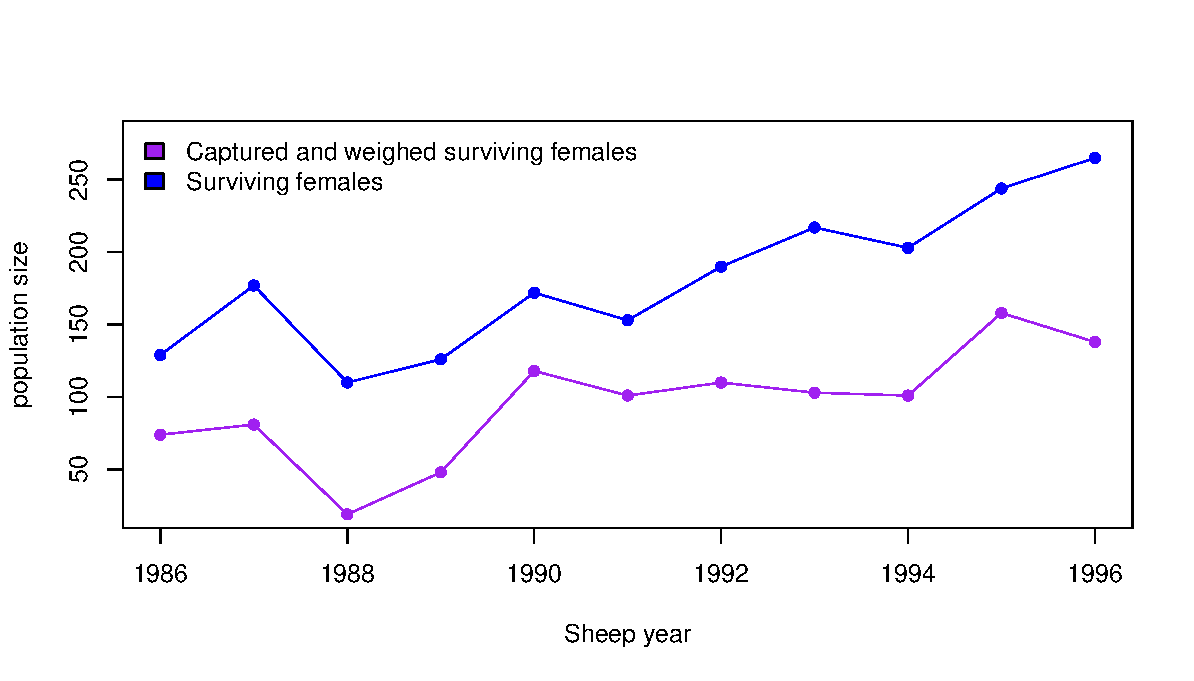
\includegraphics[scale=0.8]{dataTimeSeries.pdf}
\caption{\label{sheepTS}Counts of total and captured female \textit{Ovis aries} from the St Kirta real data, from 1986 to 1996}
\end{figure}

Our current state space model specification does not incorporate known true total population sizes, but we can still use this information to leverage a tighter prior distribution on the probability of capture. We do this by fitting a beta distribution to the observed capture probabilities at each time step (assuming independence), the results of which are illustrated by figure \ref{sheepCP}. We find that a $\text{Beta}(5.72, 5.53)$ distribution maximises the likelihood of our observed capture probabilities. The observed probability of capture is extremely low in 1988, with the cause of this drop in capture being unknown (capturing efforts are roughly consistent year to year, and experts believe there is no significant correlation between an individual's size and capture probability). The inclusion of this far lower capture probability adds to the dispersion of our prior distribution, such that it remains informative whilst reflecting our lack of certainty on the true year-on-year variation of capture probability.

\begin{figure}[H]
\centering
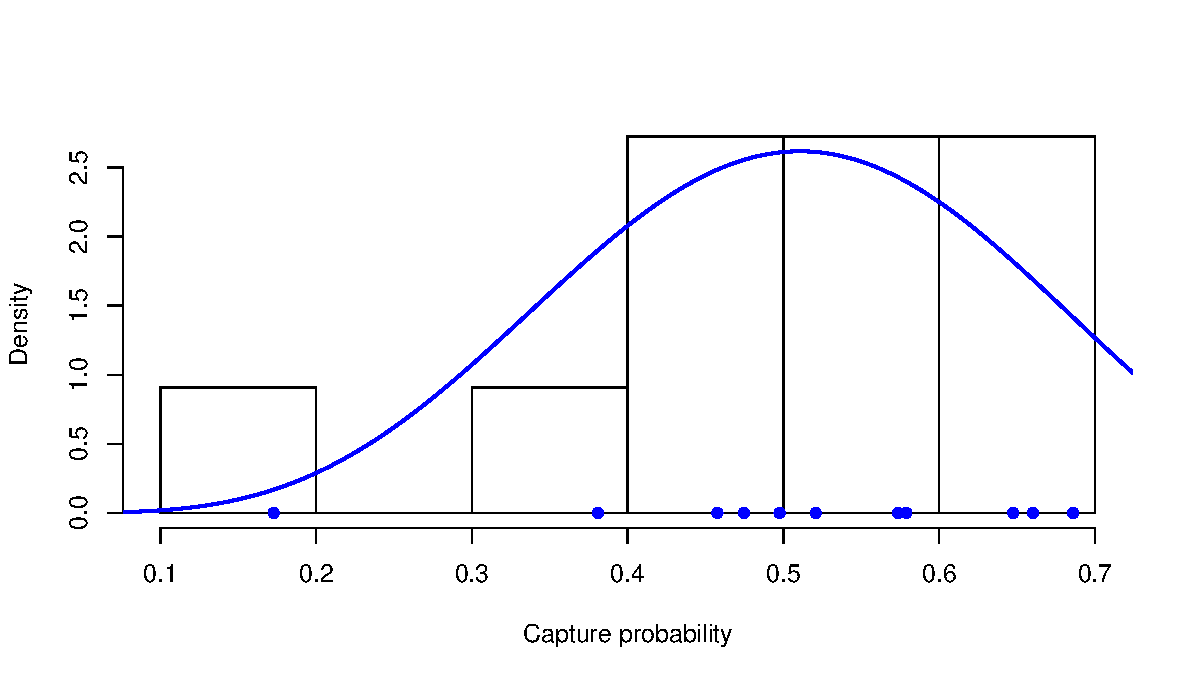
\includegraphics[scale=0.8]{captureProb.pdf}
\caption{\label{sheepCP}Observed capture probabilities for the real \textit{Ovis aries} data for the 11 years of the survey, with histogram and fitted beta distribution overlain.}
\end{figure}

We consider `shift' as a parameter in this model specification, since we are unable to approximate its true value via simulation. Whilst we wish to remain uninformative, it remains true that values of `shift' are typically centred around 0.5, and the probability of extreme values close to 0 or 1 are certainly not as likely as values around 0.5. We place a $\text{beta}(5, 5)$ prior on the `shift' parameter to reflect this. Uniform priors are placed on all other parameters, so that we may remain as close as possible to the frequentist analysis with which we hope to compare our results.

We select the observation model which considers only the observed population size at each time step, for the same reasons as the previous analysis, and keep the same specification for all of the vital rate functions. An initial estimate of the MAP was again obtained via 1000 iterations of simulated annealing, and (using 1000 calls to the particle filter for each tested value) it was found that using 50 particles resulted in a standard deviation of approximately 1.2 for the particle filter's estimate of the log likelihood of the state space model. When parameter values deviated from the simmulated annealing estimate of the MAP, the standard deviation of the estimate increased, and so 100 particles were used to run the particle MCMC, so that the standard deviation did not increase drastically when the particle filter was used to evaluate the log likelihood for proposed sets of parameter values which were less likely \textit{a posteriori}. 

Many attempts were made to use the estimated covariance structure of the posterior obtained through simulated annealing as the initial covariance for the proposal distribution. Unfortunately these attempts were largely unsuccessful. However, chains run with this proposal lead to finding a set of parameter values which had a higher posterior probability than the previously estimated MAP. To find a better initial starting proposal, we began with an isotropic Gaussian proposal where each component had the same standard deviation. We started with an extremely over-dispersed proposal with a standard deviation of 1 for each component, running 1000 iterations of the particle MCMC to estimate the acceptance rate this proposal achieved. The common standard deviation of each component was then reduced, and the pilot chain run for a further 1000 simulations in multiple iterations (each time starting at the new estimate of the MAP), until a starting standard deviation of $\frac{1}{60}$ was found to produce the desired acceptance rate (of between 0.2 and 0.25). For each iteration of this process, three to four chains were run in parallel to ensure that the estimate of the acceptance rate was roughly consistent between chains.

\subsection{Analysis}
% ANALYSIS %

Using the starting proposal which was obtained in the previous section, the final three chains were run in parallel, for 24000 iterations, updating the proposal covariance structure using the previous samples at iteration 6000 and 12000. Each chain was started at the new estimate of the MAP, such that after the burn-in period (of 14400 samples) each chain would have a different starting point and slightly different proposal covariance structure. The first chain unfortunately hit an area of low posterior density, which lead to very poor exploration of the sample space for the last few thousand iterations. For this reason the first chain was excluded, and the remaining two were used to conduct the analysis. The chains had a very low acceptance rate when excluding the burn in (3.8\% and 3.7\% respectively), and so autocorrelation between generated samples was very high. Thinning by a factor of twenty, trace plots (figure \ref{acf2}) still reveal some autocorrelation at lags as high as 15 for some parameters. After thinning we obtain 480 samples for each of the two chains, achieving an effective sample size of 85.9 and 69.1 for each chain, respectively. Including all of the chain's 9600 samples before thinning (after burn-in) only increases the effective sample size to 150.1 and 145.0 for each chain, respectively.

\begin{figure}[H]
\centering
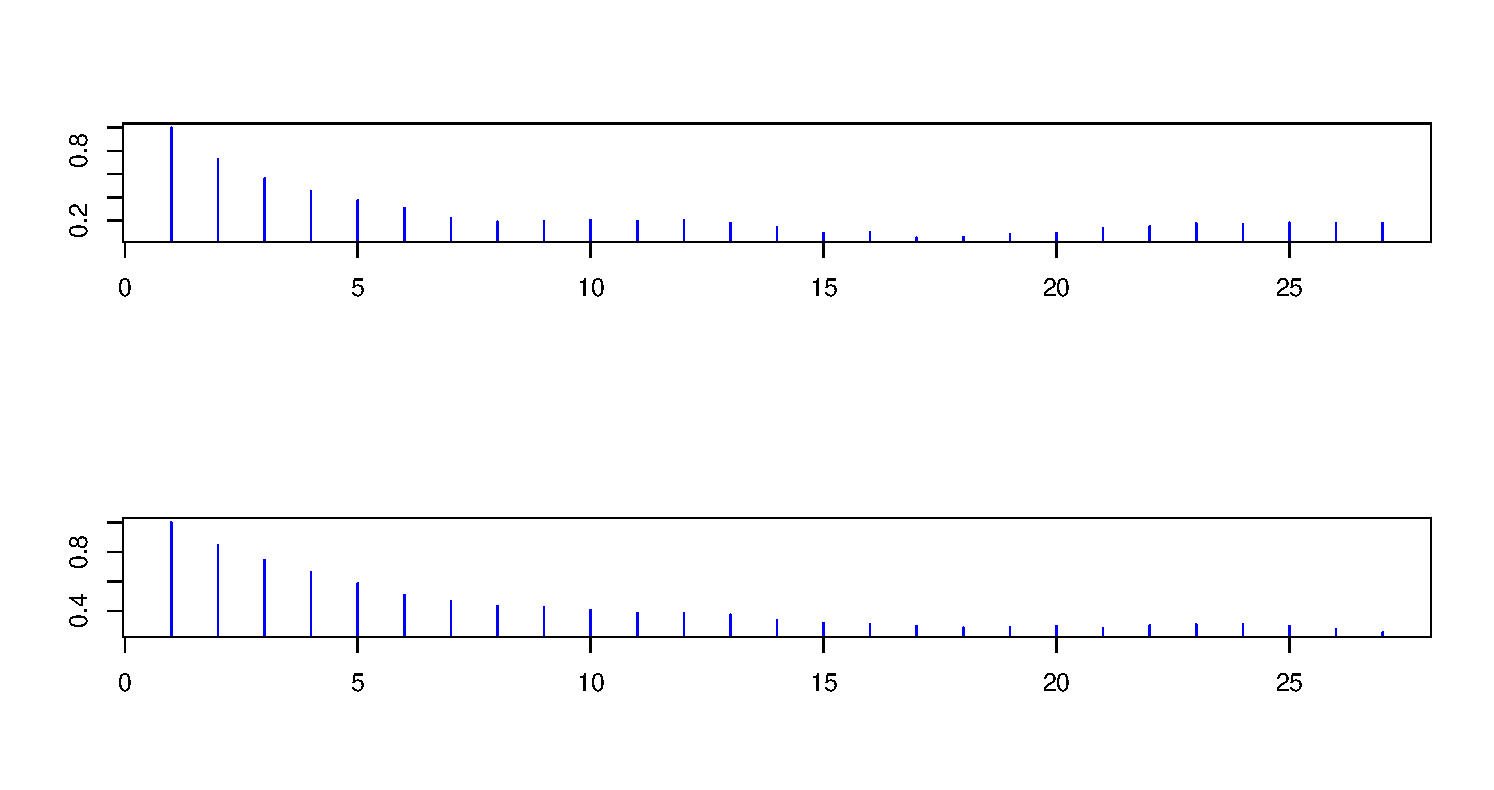
\includegraphics[scale=0.55]{chainFirst2_2.PDF}
\caption{\label{acf2}Autocorrelation plots for the first two parameters of the second chain of the \textit{Ovis aries} real data particle Markov Chain Monte Carlo output, after removing 60\% of the chain as a burn in, and thinning by a factor of 20.}
\end{figure}

\begin{figure}[H]
\centering
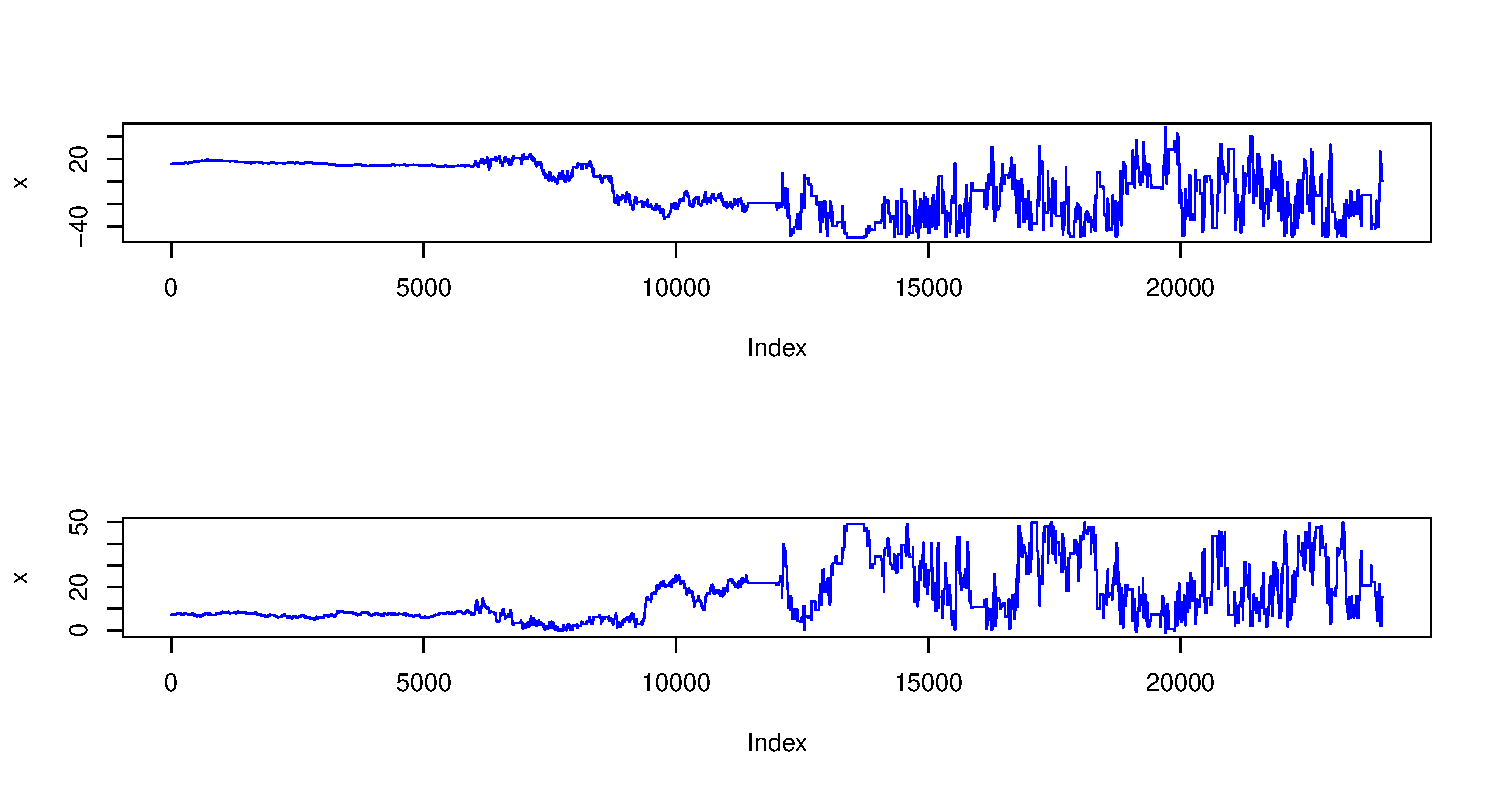
\includegraphics[scale=0.6]{chainFirst2_1.PDF}
\caption{\label{sheepTrace}Trace plots for the first two parameters of the second chain of the \textit{Ovis aries} real data particle Markov Chain Monte Carlo output}
\end{figure}

\begin{figure}[H]
\centering
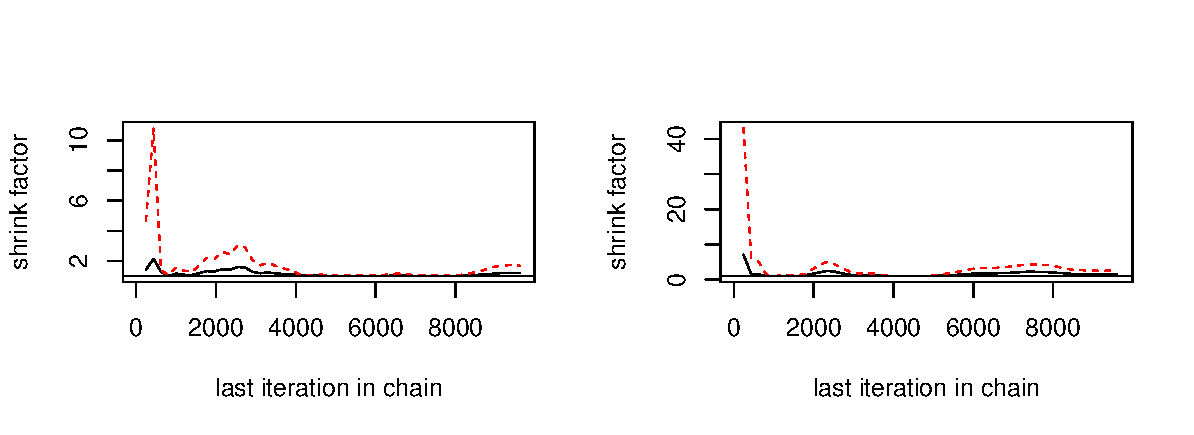
\includegraphics[scale=0.7]{GrFirst2.pdf}
\caption{\label{GRsheep}Gelman-Rubin convergence diagnostic plots for the first two parameters of the second chain of the \textit{Ovis aries} real data particle Markov Chain Monte Carlo output, after removing 60\% of the chain as a burn-in.}
\end{figure}

The trace plots (figure \ref{sheepTrace}) for the chains (before thinning or removing burn-in) indicate that convergence is less than ideal, and a Gelman-Rubin convergence diagnostic (figure \ref{GRsheep}) confirms this rather convincingly. However, the magnitude of the diagnostic is easier to identify on the full plots (which are again, all available in the supplementary materials), and is far more pronounced for the traces of other parameters. We require a far larger number of samples from the posterior distribution to make any robust inference on the nature of the posterior distribution for this model specification, and the lack of convergence of our chains should make us extremely sceptical towards using these results to draw any firm conclusions. It's very likely that this analysis also suffered from the lack of prior information, but re-running this analysis with more samples from the chains, and potentially considering far higher numbers of particles per evaluation of the log likelihood should be explored before entirely dismissing its feasibility.

\newpage
\section{Discussion}
% DISCUSSION % 

\subsection{Model extensions and revisions}
A major weakness of the presented exploration of the use of particle filtering for IPMs is the simplicity of the IPMs considered. Indeed, IPMs that consider vital rates as also being functions of population density, with year-to-year or individual random effects, such as \citet{BayesIPM} and \citet{Coulson2012}, tend to produce estimates of population growth which are less positively biased \citep{Coulson2012}. Whilst population density is not an unknown parameter, but a function of the data, its inclusion into our state space model framework could better elucidate parameter correlation structures which are more likely to agree with the underlying complicated biological relationships that generate our data. Incorporating age structure into these models could also elucidate certain previously unknown behaviours \citep{Coulson2012}, however it is clear that the speed with which these analyses can be conducted on widely available hardware must dramatically increase before such extensions may become commonplace.

We note the issues of parameter identifiability in section 4, where we saw that a lack of careful parametrisation can lead to erroneous estimation of parameter values, with prior knowledge potentially remedying this problem. An important revision to this dissertation would include re-running the analysis in section 4 to see if reasonable prior information is sufficient to remove the bias from certain parameter estimates, and if so, a sensitivity analysis should be conducted to ascertain to what extent prior knowledge is required for the state space model to be viable with commonly available computing power (perhaps even as a function of the quantity of data available, which will add information, but increase the need for computational resources).

\subsection{Suitability of Metropolis-Hastings, and the SSM parameterisation}
We observe relatively narrow posterior distributions for the parameters of interest in section 4, even with completely uninformative priors on each of these. Indeed, deviating too far from the MAP can lead to drastic drops in the value of the log posterior. Adding normal noise with a standard deviation of only 1 to the estimate of the MAP found via simulated annealing can increase the value of the negative log likelihood by an order of magnitude. Given random walk proposal Metroplis-Hastings' known inability to explore multi-modal posteriors well, it seems likely that there could be unexplored modes that are simply too far away from the MAP we find to be discovered by the MCMC. Unfortunately, restrictive priors based on frequentist analyses of other data sets could also lead to this problem, and so analysing these data sets simultaneously with the possibility of remaining uninformative \textit{a priori} would be of extreme importance. Perhaps the use of Hamiltonian Monte Carlo methods could be appropriate, if a simple enough parameterisation of the state space model is adopted, such that the gradient of the posterior could also be estimated by calling the particle filter with small variations in each dimension of the posterior space.

\subsection{Comments on data}
The data analysed in section 4 are far easier to obtain compared to typical `IPM style' data for multiple reasons. Firstly, requiring only count data allows the use of data sets where measurements of size are extremely noisy, or have been heavily rounded. When measurement error is high, models which rely on precise measurements on a continuous scale will see increasing bias in their estimations. If the measurement error is low enough that individuals can still be categorised into the correct size class, then our methodology can be used as an effective alternative. Secondly, we avoid the requirement for data which track individuals from census to census. By requiring only count data, we can fit our IPM inspired state space model to species with individuals that are hard to uniquely identitfy, without requiring the additional cost of DNA sequencing, or obtaining the lineage of any offspring which are introduced into the population. Although, we note that a formulations such as that of \citet{Coulson2012}, where the number of surviving offspring is modelled as a single entity (as opposed to the number of offspring born, and probability of offspring survival modelled separately) may be require to increase parameter identifiability before this can be pursued. Thirdly, typical maximum likelihood estimation of vital rate parameters usually requires either large population sizes, or the availability of longer times series. If simpler parameterisations of the state space model or better prior information does in fact remedy parameter identifiability, this methodology could allow the use of count data which are available for very few times steps to lead to inference of not only statistics such as growth rate or size distribution, but parameters of the vital rate functions themselves.

\subsection{Limitations, and further work}

In light of the previous sections, an obvious extension of this dissertation would be to introduce noise into the count data, and to observe the effect on the posterior distribution. This could be used to inform ecologists on which levels of noise in the raw size measurements are unlikely to lead significant bias, thus potentially allowing studies of new populations, that previously required more precise data, collected over longer periods of time with more intensive methods. It would be especially interesting to consider case studies where detection probability is low, to see if sufficient prior information on this detection probability can  elucidate parameter values for vital rate functions when the proportion of the population being sampled is low. The potential here would be significant, allowing us to perform studies on data collected via methods such as mark-recapture, with low recapture rates, instead of requiring expensive census data.

Recent advances continue to be made in statistical programming, with extremely successful forays into the use of graphics cards to perform fine grain parallelisations of advanced monte carlo algorithms, providing up to two orders of magnitude of improvement on computing time \citep{Lee, MassivelyParallel, GPUHMC}. As research continues in these fields, it is an ambition of this project to bring any advances to the field of Statistical Ecology, and specifically to the type of state space models we outline in this dissertation, through ongoing collaboration. The development of dedicated statistical software with an intuitive user interface could also reduce the need for parsing through daunting statistical papers in order to perform Bayesian analyses of survey data, facilitating the spread of new statistical developments throughout ecological literature, and making them more accessible to the field biologist.

\section{Conclusion}

This dissertation has tried to define a State Space Model specification which preserves the underlying concepts of Integral Projection Models, so that inference on parameters of vital rate functions can be analysed with a Bayesian framework, allowing parameter correlation structures to be uncovered. The theory behind the Integral Projection Model was explored, and a study of its current use and implementation in ecological literature was undertaken. A bootstrap particle filter was implemented, with a handful of modifications which alleviate the pressures of numerical underflow. This particle filter was used to perform particle Markov Chain Monte Carlo sampling from the posterior distribution of a State Space Model specification for an Integral Projection Model.

Whilst the analysis on real-data is disappointingly inconclusive due to a lack of convergence of particle Markov Chain Monte Carlo chains, and the inability of the methodology to produce reasonable estimated population growth rates from analyses on simulated data with known parameter values is disheartening, the methodology shows good potential, and certainly deserves further exploration. The results in section 5 should be tempered with the knowledge that having more computing resources, and more available time to reattempt the analysis with more informative priors with better convergence would likely lead to far more encouraging results. If the State Space Model is simplified, and computation time of each iteration of the sampling process is reduced, especially via fine grain paralellisation, then the methodology could be employed to use cheaper to collect data, over fewer time steps, to directly estimate the parameters of vital rate functions which help to describe the change of the trait-structured population's abundance over time. The exploration of parameter correlation structures in this robust context could inspire further biological research into the ecological driving forces for these relationships, furthering our understanding not only of the statistical methodology being used, but also of the real-world processes that applied statistics hopes to elucidate. Important steps in determining if the presented methodology could reach this potential include performing case studies on simulated data to ascertain if prior information can remove the observed bias in parameter estimates in section 4, and simulation studies to determine if increasing the noise in the size measurements of individuals diminishes the ability of the methodology to perform well, since its ability to work with more opportunistic or less human resource intensive data would remain the methodology's strongest selling point to the field biologist.

Biological and ecological systems are an extremely intricate web of inter-dependent hierarchical processes and interactions between many thousands of organisms. This leads to modelling their behaviour becoming a monumental task, as the vast majority of tools at our disposal are far too simple to capture all of the significant features of interest. Statistical approaches to this task will often require multiple iterations, and must be able to leverage as much cutting-edge theory and technology as possible. It is hoped that this dissertation has made a case for the continued pursuit of using particle filtering and other advanced Monte Carlo methods for Bayesian inference on ecological systems, and that finding answers to some of the questions uncovered by this dissertation's foray into State Space Models for IPMs could lead to the existence of new analytical tools to deal with smaller, noisy census data.

\clearpage

%Imports the bibliography file "sample.bib"
\bibliography{dissertation}

\end{document}